\def\sphinxdocclass{article}
\documentclass[spanish]{article}
\usepackage[utf8]{inputenc}
\usepackage{babel}
\usepackage{graphicx}
\usepackage{cmap}
\usepackage[T1]{fontenc}
\usepackage{amsmath,amssymb,amstext}
\usepackage{amsthm}
\usepackage{multirow}
\usepackage[table,xcdraw]{xcolor}
\usepackage{longtable}
\usepackage[dontkeepoldnames]{sphinx}
\usepackage{bold-extra}
\usepackage{caption}
\usepackage{subfig}
\usepackage{url}


\title{Consumo de servicios web de transferencia de estado representacional con el robot humanoide Fibonacho y sus aplicaciones}
\author{Ivan Feliciano Avelino}
\date{\today}

\graphicspath{{figures/}}


\begin{document}
\maketitle
\begin{abstract}
    Soy el resumen :)
\end{abstract}
\section{Introducción}


% Interconnection of sensing and actuating devices providing the ability to share information across platforms through a unified framework, developing a common operating picture for enabling innovative applications. This is achieved by seamless ubiquitous sensing, data analytics and information representation with Cloud computing as the unifying framework.

Actualmente existen diferentes plataformas que 
ofrecen servicios
de cómputo en la nube para solucionar problemas de 
visión computacional \cite{googlevision2018} o
procesamiento de lenguaje natural \cite{witaidocs2018} usando modelos
de aprendizaje profundo. Éstas también incluyen servicios 
para entrenar y lanzar
modelos creados por los mismos usuarios \cite{tensorflowgooglecloud2018}.
Todos estos recursos cuentan con interfaces de programación de aplicaciones
con una arquitectura de transferencia de estado representacional o REST (por sus siglas en inglés, representational state transfer) la cual 
permite que cualesquiera dispositivos que manejen el protocolo HTTP
puedan acceder a éstos.
El cómputo en la nube es un estilo de cómputo que 
permite el acceso a 
recursos informáticos a través de internet cuando un
usuario lo demanda \cite{borkofurhtarmandoescalante2010}. El aprendizaje profundo es un 
tipo
de aprendizaje automático donde las computadoras 
construyen
conceptos complejos a partir de conceptos más 
simples \cite{iangoodfellowyoshuabengioaaroncourville2017}.


%¿Qué es lo que no sabemos?\\
% El cómputo en la nube es el marco de trabajo que
% unifica los elementos que permiten que exista el
% Internet de las cosas \cite{jayavardhanagubbiarajkumarbuyyabslavenmarusicamarimuthupalaniswamia2013}. Queremos que el robot NAO, Fibonacho, 
% sea parte se esa interconexión de sensores y actuadores
% que comparten información entre plataformas
% a través de internet.
Fibonacho es un robot humanoide programable y autónomo
que a pesar de contar con
un poder de procesamiento suficiente para realizar 
tareas como
jugar un partido de fútbol con otros robots \cite{splinfo2018},
las aplicaciones modernas
exigen que los dispositivos se adapten constantemente a nuevas necesidades
de los usuarios, como el acceso a los datos
del robot a cualquier hora y desde cualquier lugar, el uso del aprendizaje profundo para resolver problemas como la 
clasificación de imágenes en múltiples categorías, encontrar
la posición de objetos en una imagen, reconocimiento
de personas y el 
procesamiento de lenguaje natural de un discurso \cite{benkehoesachinpatilpieterabbeelkengoldberg2014}.

%¿Qué pretendemos averiguar? (objetivo)

En este trabajo se integraron servicios en la nube
con el robot Fibonacho.
Los recursos son brindados por las plataformas
Google Cloud, Wit.ai, Kairos y por
el mismo Laboratorio de Algoritmos para la
Robótica.
Estos servicios en la nube permiten al robot
realizar tareas como el procesamiento de lenguaje
natural de un discurso oral, el procesamiento 
de imágenes para reconocimiento de rostros
y objetos y la clasificación de
imágenes en escenarios.
\section{Antecedentes}


\subsection{Robot NAO}
NAO es un robot humanoide autónomo y programable desarrollado por la empresa de
Aldebaran Robotics.

El robot NAO mide 57.3 cm de altura, 27.3 cm de ancho, y pesa menos de 4.3 kg.
El cuerpo está construido de un material de plástico y tiene una batería de ion
de litio que lo abastece para un uso normal de aproximadamente
90 minutos o 60 en un modo activo.

Las versiones \textit{V5} y \textit{V4} tiene una CPU Atom de 1.6 GHz, 1 GB de RAM, una
memoria flash de 2 GB y una micro SDHC de 8GB.

Se comunica remotamente con otros dispositivos mediante WiFi o por medio de un
cable Ethernet. También cuenta con un puerto USB cuyo principal uso es para
añadir un dispositivo como un sensor 3D o un Arduino.

Para la parte multimedia, el robot está equipado con un sistema de transmisión
estéreo compuesto por dos bocinas en las orejas. Dos micrófonos en la cabeza
con un paso de banda eléctrico entre 300Hz y 8kHz. Dos cámaras idénticas están
localizadas en la parte anterior de la cabeza. Éstas proveen imágenes con una
resolución de hasta 1280px $\times$ 960px y 30 cuadros por segundo.

Cuenta con diodos emisores de luz distribuidos entre la cabeza, orejas, ojos, pecho y pies. Cada
uno de estos últimos cuenta con resistencias sensibles a la fuerza, que son
sensores encargados de medir la resistencia al cambio de acuerdo a una presión
aplicada. Trabajan en un rango de 0 N a 25 N.

En el torso está localizada una unidad de medición inercial, compuesta por un
girómetro y un acelerómetro, la cual permite una estimación de la velocidad
y postura del torso.

El robot está equipado con dos sensores ultrasónicos, que sirven para estimar
la distancia a obstáculos. Dependiendo de la versión del robot, el rango de
detección varía de 0.20 cm a 0.80 cm en la última versión y 0.25 cm a 2.55 cm
en versiones anteriores. Cuando la distancia es menor al límite inferior de
cada versión, el robot únicamente sabe que hay un obstáculo presente.
Tiene un cono efectivo de 60 grados.

Entre los sensores restantes están los de posición de las articulaciones, los
de contacto y los táctiles. Los dos últimos están en la cabeza, manos, pecho y
pies.

Tiene en total 25 articulaciones repartidas entre la cabeza, brazos,
piernas y pelvis. Todas las articulaciones cuentan con controladores de posición.
Dada una articulación que enlaza dos partes del cuerpo del robot, la parte
del cuerpo que está más cerca del tronco se considera fija y la parte que está
más lejos  es la que rota alrededor de los ejes de la articulación.
Para realizar una rotación de las partes del cuerpo, definimos un sistema
de referencia en cada articulación.
En el sistema de referencia se tienen tres ángulos de rotación:
\textit{roll} (dirección), \textit{pitch} (elevación) y \textit{roll} (alabeo).
Las rotaciones \textit{roll}, son
alrededor del eje X, las \textit{pitch}  sobre Y y \textit{yaw} con respecto a Z. La figura
 \ref{\detokenize{chapter_one/naoqi:rollpitchyaw-frame}} muestra el sistema de referencia.

\begin{figure}[htbp]
\centering


\noindent\includegraphics[scale=0.7]{{rollPitchYaw_frame}.png}
\caption{Sistema de referencia de los ángulos de rotación}\label{\detokenize{chapter_one/naoqi:rollpitchyaw-frame}}\end{figure}

En la figura \ref{\detokenize{chapter_one/naoqi:nao-config}} se muestran algunos de los componentes del robot NAO.

\begin{figure}[htbp]
\centering


\noindent\includegraphics[scale=0.4]{{nao_config}.png}
\caption{Componentes del robot NAO}\label{\detokenize{chapter_one/naoqi:nao-config}}\end{figure}


\subsection{NAOqi}
\label{\detokenize{chapter_one/naoqi:naoqi}}
NAOqi es el nombre del software principal que corre sobre el robot y lo
controla.El marco de trabajo de NAOqi es el marco de trabajo de programación
usado para programar robots de Aldebaran. Brinda
soluciones a necesidades básicas de la robótica como el paralelismo, el manejo
de recursos, la sincronización y los eventos.

\subsubsection{Interfaces de programación de aplicaciones (API) de NAOqi}
\label{\detokenize{chapter_one/naoqi:interfaces-de-programacion-de-aplicaciones-api-de-naoqi}}
NAOqi cuenta con bastantes API divididas en grupos de acuerdo a las
funcionalidades que ofrecen. 
% A continuación se enlistan algunos grupos
% y sólo se describen de manera breve aquellas API,
% que se utilizaron en el desarrollo de este proyecto.

% NAOqi viene con una lista de módulos centrales que están disponibles siempre.
% Cada módulo cuenta con una lista de métodos por defecto.


% \subparagraph{ALMemory.}
% \label{\detokenize{chapter_one/naoqi:id1}}
% Es una memoria centralizada usada para almacenar toda la información importante
% relacionada con la configuración del hardware del robot.
% \texttt{ALMemory} provee información acerca del estado actual de actuadores y sensores.

% De manera más específica, \texttt{ALMemory} es un mapa no ordenado de la biblioteca
% \textbf{boost}. El mapa está compuesto por contenedores genéricos (\texttt{ALValues}).

NAOqi contiene un grupo de módulos enfocados a los movimientos del robot,
ya sea para navegar de manera segura, cambiar entre posturas predefinidas,
realizar movimientos de forma autónoma y hasta generar movimientos
personalizados.


\subparagraph{ALMotion.}
\label{\detokenize{chapter_one/naoqi:almotion}}
Es la principal herramienta para permitir que el robot se mueva.

Contiene cuatro principales grupos de métodos para controlar:
\begin{itemize}
\item {} 
la rigidez de articulaciones, básicamente si un motor está prendido o apagado.

\item {} 
la posición de articulaciones, para la planeación de trayectorias (interpolación) y cambios en los valores de los motores como respuesta a datos en sensores (control reactivo).

\item {} 
el caminado, control de distancia y velocidad, posición en un ambiente, etc.

\item {} 
efector del robot en el espacio cartesiano, determinar el movimiento de una cadena de articulaciones para lograr que un actuador se ubique en una posición concreta (cinemática inversa).

\end{itemize}

El eje \textbf{X} es positivo con respecto al frente del robot, el eje \textbf{Y} de
derecha a izquierda y el \textbf{Z} es vertical.
La figura \ref{\detokenize{chapter_one/naoqi:almotionaxis}} muestra la definición de los ejes con respecto al robot.
% \subparagraph{\textbf{Sistema Internacional de Unidades}}
% \label{\detokenize{chapter_one/naoqi:sistema-internacional-de-unidades}}
El módulo de \texttt{ALMotion} usa el Sistema Internacional de Unidades (metros,
segundos, radianes, etc).
\begin{figure}[!ht]
\centering


\noindent\includegraphics[scale=0.40]{{almotionaxis}.png}
\caption{Sistema de ejes sobre los que el robot ejecuta movimientos}\label{\detokenize{chapter_one/naoqi:almotionaxis}}\end{figure}




% \paragraph{Audio}
% \label{\detokenize{chapter_one/naoqi:audio}}
NAOqi cuenta con componentes de software para el audio; para
manejar la salida o entrada a través de sus bocinas y micrófonos,
para la detección y localización de sonidos,  y para el manejo del lenguaje.


\subparagraph{ALTextToSpeech.}
\label{\detokenize{chapter_one/naoqi:altexttospeech}}
Este módulo permite al robot hablar. Envía órdenes a un componente que
convierte texto a un discurso hablado, y autoriza la personalización de la voz.
El resultado de la síntesis es enviado a las bocinas del robot.


\subparagraph{ALAnimatedSpeech.}
\label{\detokenize{chapter_one/naoqi:alanimatedspeech}}
El módulo \texttt{ALAnimatedSpeech} brinda la posibilidad de hacer que el robot hable
de una manera expresiva. El funcionamiento de este módulo es como sigue:
\begin{enumerate}
\item {} 
\texttt{ALAnimatedSpeech} recibe texto que puede ser \textit{anotado} con \textit{instrucciones}.

\item {} 
Divide el texto en subcadenas de menor tamaño a la original.

\item {} 
Analiza el texto y anota las cosas que reconoce para realizar movimientos de acuerdo al contexto.

\item {} 
Cualquier parte del texto que no esté anotado con animaciones se llena con \textit{modos de lenguaje corporal}.

\item {} 
El módulo prepara al robot para ejecutar cada instrucción para que estas sean llamadas tan pronto como se necesiten. Esto permite que el discurso y las instrucciones estén sincronizados.

\item {} 
\texttt{ALAnimatedSpeech} hace que el robot diga el texto y se mantenga al tanto del discurso para lanzar las instrucciones en el momento correcto.

\end{enumerate}


\subparagraph{ALAudioRecorder.}
\label{\detokenize{chapter_one/naoqi:alaudiorecorder}}
\texttt{ALAudioRecorder} provee servicios de grabación en archivos «WAV»
u «OGG» a partir de las señales recibidas de los micrófonos del robot.

Este módulo depende la biblioteca de Linux SDNFile para
codificar de manera eficiente entradas de audio en tiempo real.

Las capacidades de grabación están limitadas a los siguientes
formatos:
\begin{itemize}
\item {} 
cuatro canales 48000 Hz para OGG y WAV

\item {} 
un canal (anterior, posterior, izquierda o derecha) para OGG y WAV.

\end{itemize}

%\paragraph{Vision}
% \label{\detokenize{chapter_one/naoqi:vision}}
Los módulos de visión provistos por NAOqi se encargan del manejo de video e
imágenes, detección de objectos predefinidos en video, y cuenta con herramientas
para crear una memoria visual donde aprenda y reconozca ciertos patrones,
y herramientas para navegación, usar una imagen como brújula, entre otras.


\subparagraph{ALVideoDevice.}
\label{\detokenize{chapter_one/naoqi:alvideodevice}}
Este módulo es responsable de proveer, de una manera eficiente, imágenes de la
cámara del robot a todos los módulos que las procesan, como \texttt{ALFaceDetection}
o \texttt{ALVisionRecognition}.


% \subparagraph{Uso}
% \label{\detokenize{chapter_one/naoqi:id2}}
Para empezar a utilizar este módulo es necesario seguir los siguientes pasos:
\begin{enumerate}
\item {} 
Hacer que tu módulo de visión se suscriba al proxy de \texttt{ALVideoDevice}, llamando el método \texttt{subscribeCamera()} y pasando como parámetros la resolución, espacio de color y tasa de fotogramas.

\item {} 
En el bucle del proceso principal, obtener una imagen llamando a los métodos \texttt{getImageLocal()} o \texttt{getImageRemote()} (dependiendo si el módulo es local o remoto).

\item {} 
Liberar la imagen llamando \texttt{releaseImage()}.

\item {} 
Cuando se detiene el módulo, se llama \texttt{unsubscribe()} después de salir de bucle principal.

\end{enumerate}

% \paragraph{Sensores}
% \label{\detokenize{chapter_one/naoqi:sensores}}
% Existen numerosos sensores en el robot NAO. NAOqi ofrece módulos para interactuar
% con el robot a través de algunos de ellos, o manejar eventos cuando estos
% cambian valores.


% \subparagraph{ALSonar.}
% \label{\detokenize{chapter_one/naoqi:alsonar}}
% El módulo de \texttt{ALSonar} obtiene valores de los sensores ultrasónicos desde
% \texttt{ALMemory}, procesa esa información y lanza eventos de acuerdo con la situación.
% Para ahorrar energía, los sensores ultrasónicos no están activados por defecto.

% Los valores actuales de los sensores se pueden recuperar desde \texttt{ALMemory} a través del método \texttt{getData()} de \texttt{ALMemory}.


%\subparagraph{Uso}
%\label{\detokenize{chapter_one/naoqi:id3}}
% El hardware de los sensores no se inicia de manera automática. Para empezar,
% es necesario suscribirse al módulo de \texttt{ALSonar} a través del método \texttt{subscribe()}.
% Hacer esto prende los sensores ultrasónicos.
% Para apagar los sensores, se debe cancelar la suscripción con el método
% \texttt{unsubscribe()} de \texttt{ALSonar}.


% \subsubsection{SDK de Python}
% \label{\detokenize{chapter_one/naoqi:sdk-de-python}}
% La API de Python para los robots de Aldebaran permite:
% \begin{itemize}
% \item {} 
% usar la API de C++ desde una máquina remota

% \item {} 
% crear módulos de Python que puedan ejecutarse remotamente o localmente en el robot.

% \end{itemize}

% Un programa muy básico en Python para los robots tiene la siguiente estructura:
% \begin{itemize}
% \item {} 
% Primero importar \texttt{ALProxy}

% \item {} 
% Instanciar un objecto de \texttt{ALProxy} para el módulo que se quiere usar

% \item {} 
% Llamar un método

% \end{itemize}

% El siguiente fragmento de código es un ejemplo de un programa que hace al robot
% caminar sobre su eje \textbf{X} durante tres segundos:

% \begin{sphinxVerbatim}[commandchars=\\\{\}]
% \PYG{c+c1}{\PYGZsh{} encoding: utf\PYGZhy{}8}
% \PYG{k+kn}{import} \PYG{n+nn}{time}
% \PYG{k+kn}{from} \PYG{n+nn}{naoqi} \PYG{k}{import} \PYG{n}{ALProxy} \PYG{c+c1}{\PYGZsh{} Importa ALProxy}

% \PYG{n}{motion\PYGZus{}proxy} \PYG{o}{=} \PYG{n}{ALProxy}\PYG{p}{(}\PYG{l+s+s2}{\PYGZdq{}}\PYG{l+s+s2}{ALMotion}\PYG{l+s+s2}{\PYGZdq{}}\PYG{p}{,} \PYG{l+s+s2}{\PYGZdq{}}\PYG{l+s+s2}{\PYGZlt{}IP del robot\PYGZgt{}}\PYG{l+s+s2}{\PYGZdq{}}\PYG{p}{,} \PYG{l+m+mi}{9559}\PYG{p}{)} \PYG{c+c1}{\PYGZsh{} Crear un proxy al módulo ALMotion}

% \PYG{n}{motion\PYGZus{}proxy}\PYG{o}{.}\PYG{n}{wakeUp}\PYG{p}{(}\PYG{p}{)} \PYG{c+c1}{\PYGZsh{} Utiliza un método de ALMotion para cambiar la postura del robot}
% \PYG{n}{x} \PYG{o}{=} \PYG{l+m+mf}{0.5}
% \PYG{n}{y} \PYG{o}{=} \PYG{l+m+mf}{0.0}
% \PYG{n}{theta} \PYG{o}{=} \PYG{l+m+mf}{0.0}

% \PYG{n}{motion\PYGZus{}proxy}\PYG{o}{.}\PYG{n}{moveToward}\PYG{p}{(}\PYG{n}{x}\PYG{p}{,} \PYG{n}{y}\PYG{p}{,} \PYG{n}{theta}\PYG{p}{)}
% \PYG{n}{time}\PYG{o}{.}\PYG{n}{sleep}\PYG{p}{(}\PYG{l+m+mi}{3}\PYG{p}{)}

% \PYG{n}{motion\PYGZus{}proxy}\PYG{o}{.}\PYG{n}{stopMove}\PYG{p}{(}\PYG{p}{)}

% \PYG{n}{motion\PYGZus{}proxy}\PYG{o}{.}\PYG{n}{rest}\PYG{p}{(}\PYG{p}{)}
% \end{sphinxVerbatim}


% \subsubsection{SDK de JAVA}
% \label{\detokenize{chapter_one/naoqi:sdk-de-java}}
% El SDK de Java provee una API para llamar servicios remotos, crear nuevos
% servicios y reaccionar a eventos.

% El SDK está basado en la biblioteca \textbf{libqi-java}, la cual utiliza el
% \textbf{marco de trabajo qi}. Es una nueva arquitectura, que permite utilizar la API de NAOqi con una sintaxis
% nueva y sencilla.En vez de crear un proxy a un módulo, se crea una sesión y se solicita un servicio. El resultado de esto es un objeto con los mismos métodos del
% módulo que se desea.

% Existe un archivo \texttt{.jar} por cada plataforma y versión de NAOqi. Éste
% permite usar la API de C++ de Aldebaran o crear servicios
% personalizados, y ejecutarlos desde un dispositivo remoto o directamente en el
% robot.

% Para compilar una aplicación desde la línea de comandos, se realiza los
% siguiente

% \begin{sphinxVerbatim}[commandchars=\\\{\}]
% \PYG{c+c1}{\PYGZsh{} Compilación}
% javac \PYGZhy{}cp /ruta/a/java\PYGZhy{}naoqi\PYGZhy{}sdk\PYGZhy{}\PYGZlt{}version\PYGZgt{}\PYGZhy{}\PYGZlt{}platform\PYGZgt{}.jar MyApp.java
% \PYG{c+c1}{\PYGZsh{} Ejecución}
% java \PYGZhy{}cp /ruta/a/java\PYGZhy{}naoqi\PYGZhy{}sdk\PYGZhy{}\PYGZlt{}version\PYGZgt{}\PYGZhy{}\PYGZlt{}platform\PYGZgt{}.jar:. MyApp
% \end{sphinxVerbatim}

% Hay dos conceptos importantes que se deben conocer que permiten la comunicación
% con el robot: \texttt{Application} y \texttt{Session}.

% Una \texttt{Application} es responsable de inicializar el marco de trabajo
% y conectarse a una sesión. Una \texttt{Session} es lo que permite conectarse a
% servicios local o remotamente.

% Por defecto, el URL de la sesión está configurado para ser
% \texttt{127.0.0.1:9559}. Pero éste se puede cambiar en los argumentos del
% constructor de \texttt{Application}.

% En el SDK de Java, existen clases para cada servicio. Esto último significa
% que se debe crear una instancia de cada servicio que se desea para que sea
% posible llamar sus métodos.

% El siguiente ejemplo muestra como hacer que el robot diga la frase
% “Cells Interlinked Within Cells Interlinked” usando \texttt{ALTextToSpeech}.

% \begin{sphinxVerbatim}[commandchars=\\\{\}]
% \PYG{k+kd}{public} \PYG{k+kd}{static} \PYG{k+kt}{void} \PYG{n+nf}{main}\PYG{o}{(}\PYG{n}{String}\PYG{o}{[}\PYG{o}{]} \PYG{n}{args}\PYG{o}{)} \PYG{o}{\PYGZob{}}
%   \PYG{c+c1}{// Se define el URL del robot}
%   \PYG{n}{String} \PYG{n}{robotUrl} \PYG{o}{=} \PYG{l+s}{\PYGZdq{}tcp://192.168.4.220:9559\PYGZdq{}}\PYG{o}{;}
%   \PYG{n}{Application} \PYG{n}{application} \PYG{o}{=} \PYG{k}{new} \PYG{n}{Application}\PYG{o}{(}\PYG{n}{args}\PYG{o}{,} \PYG{n}{robotUrl}\PYG{o}{)}\PYG{o}{;}
%   \PYG{k}{try}\PYG{o}{\PYGZob{}}
%       \PYG{c+c1}{// Se inicial la aplicación y se genera una sesión}
%       \PYG{n}{application}\PYG{o}{.}\PYG{n+na}{start}\PYG{o}{(}\PYG{o}{)}\PYG{o}{;}
%       \PYG{c+c1}{// La sesión puede recuperarse a través del método siguiente}
%       \PYG{c+c1}{// application.session();}
%       \PYG{c+c1}{// Crear un objeto de ALTextToSpeech y lo enlaza con la sesión actual}
%       \PYG{n}{ALTextToSpeech} \PYG{n}{tts} \PYG{o}{=} \PYG{k}{new} \PYG{n}{ALTextToSpeech}\PYG{o}{(}\PYG{n}{application}\PYG{o}{.}\PYG{n+na}{session}\PYG{o}{(}\PYG{o}{)}\PYG{o}{)}\PYG{o}{;}
%       \PYG{c+c1}{// El robot dice la frase}
%       \PYG{n}{tts}\PYG{o}{.}\PYG{n+na}{say}\PYG{o}{(}\PYG{l+s}{\PYGZdq{}Cells Interlinked Within Cells Interlinked\PYGZdq{}}\PYG{o}{)}\PYG{o}{;}
%   \PYG{o}{\PYGZcb{}}
%   \PYG{k}{catch}\PYG{o}{(}\PYG{n}{Exception} \PYG{n}{e}\PYG{o}{)}\PYG{o}{\PYGZob{}}
%       \PYG{c+c1}{// La aplicación no pudo iniciar.}
%       \PYG{n}{e}\PYG{o}{.}\PYG{n+na}{printStackTrace}\PYG{o}{(}\PYG{o}{)}\PYG{o}{;}
%   \PYG{o}{\PYGZcb{}}
% \PYG{o}{\PYGZcb{}}
% \end{sphinxVerbatim}



\section{Servicios Web REST}
\label{\detokenize{chapter_one/rest:arquitecturas-de-servicios-de-transferencia-de-estado-representacional}}\label{\detokenize{chapter_one/rest::doc}}


\subsection{Transferencia de Estado Representacional (REST)}
\label{\detokenize{chapter_one/rest:transferencia-de-estado-representacional-rest}}
% En el año 2000, después de que la crisis de la escalabilidad de la web se
% evitó, Fielding llamó y describió al estilo arquitectónico de la web en su
% trabajo doctoral. \sphinxstylestrong{Transferencia de Estado Representacional} (REST por
% sus siglas en inglés) fue el nombre que Fielding dio a su descripción del
% estilo arquitectónico de la web, que está compuesto por las restricciones
% mencionadas previamente.

La Transferencia de Estado Representacional es un estilo de arquitectura de software.
Este estilo es
una abstracción de elementos arquitectónicos dentro de un sistema de hipermedia
distribuido como es la Web. REST ignora los detalles de la implementación de
componentes y sintaxis de protocolos de manera que pueda enfocarse en los
papeles de los componentes, las restricciones sobre su interacción con otros
componentes, y la interpretación de elementos de datos significativos.
Abarca las limitaciones fundamentales sobre los componentes, conectores y datos
que definen las bases de la arquitectura web y, por lo tanto, la esencia de su
comportamiento como una aplicación basada en red. REST no es un estándar, sin
embargo sí un conjunto de restricciones. No está atado al protocolo HTTP,
pero a menudo se asocia con éste.


\subsubsection{API REST}
\label{\detokenize{chapter_one/rest:api-rest}}
Un \sphinxstyleemphasis{servicio web} es un sistema de software diseñado para admitir
la interacción interoperable de una máquina a otra  máquina a través de una red.
Programas cliente usan \sphinxstyleemphasis{interfaces de programación de aplicaciones} (API
por sus siglas en inglés) para comunicarse con servicios web. Una API expone un conjunto de datos y funciones para facilitar
interacciones entre programas de computadora y permitiendo que
intercambien información.

\begin{figure}[htbp]
\centering


\noindent\sphinxincludegraphics[scale=0.60]{{web_service_cycle}.png}
\caption{Una API web es el frente de un servicio web, escuchando y respondiendo las peticiones de los cliente directamente.}\label{\detokenize{chapter_one/rest:web-service-cycle}}\end{figure}

El estilo arquitectónico REST se aplica comúnmente al diseño de API para
servicios web modernos. Una API web que sigue el estilo REST es una API REST.
Tener una API REST hace a un servicio web RESTful. Una API REST está formada de
recursos entrelazados.\\

REST es una arquitectura basada en recursos. Se accede a un recurso a través
de una interfaz común basada en los métodos estándar de HTTP. REST
solicita a los desarrolladores usar métodos HTTP explícitamente
y de una forma que sea consistente con la definición del protocolo.
Cada recurso se identifica con un URL. Todos los recursos deben soportar
las operaciones HTTP más comunes, además REST permite que ese recurso
tenga diferentes representaciones, por ejemplo, texto, XML, JSON, etc.
El cliente REST puede solicitar una representación en específico por
medio del protocolo HTTP. El cuadro \ref{\detokenize{chapter_one/rest:rest-struct}} describe
los elementos usados en REST.



\begin{table}
\centering
\caption{Elementos de REST}\label{\detokenize{chapter_one/rest:rest-struct}}
\begin{tabulary}{\linewidth}[t]{|T|T|}
\hline
\sphinxstylethead{ 
Elemento
\unskip}\relax &\sphinxstylethead{ 
Descripción
\unskip}\relax \\
\hline
Recurso
&
Objetivo conceptual de una referencia de hipertexto. Por ejemplo: podcast.
\\
\hline
Identificador de recurso
&
Un URL que identifica un recurso en específico. Por ejemplo: \sphinxurl{http://convoynetwork.com/podcast/123}
\\
\hline
Metadatos del recurso
&
Información que describe al recurso. Por ejemplo: autor, etiqueta, etc.
\\
\hline
Representación
&
El contenido del recurso. Por ejemplo: un JSON, un HTML o una imagen JPEG.
\\
\hline
Metadatos de la representación
&
Información que describe como procesar la representación. Por ejemplo: tipo de medio, fecha, etc.
\\
\hline
Datos de control
&
Información que describe cómo optimizar el procesamiento de respuesta. Por ejemplo: if-modified-since, cache-control-expiry.
\\
\hline
\end{tabulary}
\end{table}

\section{Servidor REST}
Se creó un servidor el cual es cliente de los servicios web de terceros y a la vez
ofrece los mantenidos por el LAR.
El resultado de la unión cliente-servidor se
entrega por medio de una
API REST.
Todos los servicios brindados tienen en común que están basados en modelos de
aprendizaje automático, específicamente de aprendizaje profundo. Estos dan solución
a problemas de visión computacional como la detección de rostros o el
reconocimiento óptico de caracteres, el reconocimiento
de voz, el procesamiento de lenguaje natural y la traducción automática
neuronal. A continuación se enlistan los servicios de terceros que el servidor
consume.
\begin{itemize}
\item {} 
Google Cloud Vision, permite comprender el contenido de una imagen. Son dos las funcionalidades ocupadas; el etiquetado de imágenes en miles de categorías y el reconocimiento óptico de caracteres (OCR).

% \item {} 
% \url{https://cloud.google.com/speech/}{API Speech de Google Cloud}, convierte audio a texto.

\item {} 
Google Cloud Translation, se encarga de traducir una cadena arbitraria en cualquier idioma admitido.

\item {} 
Kairos, es una API de reconocimiento facial. Esta cuenta con varios métodos, de los cuales se utilizaron \sphinxstyleemphasis{enroll} y \sphinxstyleemphasis{recognize}. El primero para añadir a un nuevo rostro a una base de datos junto con un identificador, el segundo para encontrar a un usuario cuya cara ha sido almacenada.

\item {} 
Wit.ai, un servicio para procesamiento de lenguaje natural capaz de convertir oraciones en información estructurada.

\end{itemize}


Los servicios mantenidos por el LAR son dos modelos de TensorFlow.
El primero permite la detección de objetos en imágenes y es parte
de la API de detección de objetos de TensorFlow. El segundo
servicio es un clasificador de imágenes en cuatro categorías.

El servidor mantiene la ejecución de un contenedor de
Docker en el que se encuentra corriendo una aplicación web desarrollada en Python.
Dicha aplicación es la API REST que se comunica con el robot y dispositivos
que soliciten los recursos. 
La figura \ref{\detokenize{chapter_two/desc_cloudnao:cn-server-lar-diagram}} muestra de manera general la estructura del
servidor.

\begin{figure}[htbp]
\centering


\noindent\sphinxincludegraphics[scale=0.35]{{CN_server_lar_diagram}.png}
\caption{Diagrama del servidor}\label{\detokenize{chapter_two/desc_cloudnao:cn-server-lar-diagram}}\end{figure}

\section{API REST}

Esta interfaz es el producto de la integración de modelos de aprendizaje
automático
enfocados a casos de uso relacionados con la robótica.
% Es uno de los componentes más importantes en toda la arquitectura,
% es el que une los servicios web de
% terceros, los módulos mantenidos por el LAR y los entrega en una sola API.

La API REST  permite integrar dentro de una aplicación un
conjunto de herramientas para el análisis de imágenes.
Todas éstas basadas en modelos de aprendizaje automático. El URL base al
que todos los recursos son relativos es \sphinxcode{http://132.248.180.17/}.

La API tiene tres recursos:
\begin{itemize}
\item {} 
\sphinxcode{/register}: para que un nuevo usuario se registre y pueda ocupar los otros recursos. Envía una dirección de correo y una contraseña.

\item {} 
\sphinxcode{/refreshtoken}: para que el usuario pueda obtener un nuevo token de acceso al enviar los datos con los que se registró.

\item {} 
\sphinxcode{/vision}: el recurso más importante. Se le solicita que haga procesamiento de imágenes.

\end{itemize}

\subsection{Recurso /vision}
\label{\detokenize{chapter_two/desc_cloudnao:vision}}
Este recurso es el encargado de la detección de características en una
imagen. Estas características son: la \sphinxstylestrong{detección de objetos}, el
\sphinxstylestrong{reconocimiento de rostros}, de personas previamente guardadas o de
nuevos sujetos para su almacenamiento, la \sphinxstylestrong{clasificación en cuatro escenarios}, lugares
dentro del laboratorio de algoritmos para la robótica, la
\sphinxstylestrong{detección de etiquetas o categorías}
y la \sphinxstylestrong{traducción de texto encontrado en una imagen}.

En este recurso la única forma de persistencia de datos es al guardar el
rostro de una nueva persona para su posterior reconocimiento.


\subsubsection{POST /vision}
\label{\detokenize{chapter_two/desc_cloudnao:post-vision}}

El único método definido para el recurso \texttt{/vision}
es POST. Se envía a la API una imagen ya sea codificada en base 64 o mediante su URL y
las características que se desean obtener. Las características disponibles
son las siguientes:

\begin{itemize}
    \item{}
    \sphinxcode{FACE\_ENROLL}:
Detecta un rostro en la imagen y
con un identificador enviado en
el cuerpo de la petición se
almacena en una galería de
Kairos. Se emplea
\texttt{/enroll}
de Kairos.
\item{}
\sphinxcode{FACE\_RECOGNITION}:
Encuentra rostros dentro de una
imagen y los relaciona con los
rostros similares previamente
guardados en una galería de
Kairos. Usa
\texttt{/recognize}
de la API de Kairos.
\item{}
\sphinxcode{OBJECT\_DETECTION}:
Busca objetos en una la imagen,
usa la API de detecctión de objetos de TensorFlow.
Regresa las coordenadas de un
cuadro delimitador para cada
objeto detectado.
\item{}
\sphinxcode{LABELS\_DETECTION}:
Clasifica una imagen en distintas
categorías. Se vale de la API de Google Cloud Vision
\item{}
\sphinxcode{OCR\_TRANSLATION}:
Lleva a cabo el reconocimiento de
texto en una imagen, para
posteriormente traducirlo.
Utiliza la API de Google Cloud
Vision
para el reconocimiento de
caracteres y la de Google Cloud
Translation
para la segunda parte del proceso.
\item{}
\sphinxcode{CLASSIFY\_INDOOR\_SCENES}:
Clasifica una imagen en cuatro
categorías. Cada categoría es un
lugar dentro del área del LAR.

\end{itemize}


\paragraph{Mensaje de solicitud}
\label{\detokenize{chapter_two/desc_cloudnao:peticion}}

\subparagraph{Headers.}
\label{\detokenize{chapter_two/desc_cloudnao:headers}}
En los encabezados de la petición debe de ir el tipo de contenido que se envía
y un token de acceso único para cada usuario registrado. Esto último
simplemente es para evitar que cualquiera pueda hacer peticiones a la API.

\begin{sphinxVerbatim}[commandchars=\\\{\}]
\PYG{n}{Content}\PYG{o}{\PYGZhy{}}\PYG{n}{Type}\PYG{p}{:} \PYG{n}{application}\PYG{o}{/}\PYG{n}{json}
\PYG{n}{Authorization}\PYG{p}{:} \PYG{n}{ACCESS\PYGZus{}TOKEN}
\end{sphinxVerbatim}


\subparagraph{\sphinxstylestrong{Cuerpo.}}
\label{\detokenize{chapter_two/desc_cloudnao:body}}
En el cuerpo del mensaje se envía un JSON con la siguiente estructura. En la tabla 
\ref{tab:body_json_schema_request} se describen los atributos del JSON.

\begin{sphinxVerbatim}[commandchars=\\\{\}]
\PYG{p}{\PYGZob{}}
  \PYG{l+s+s2}{\PYGZdq{}imageContent\PYGZdq{}}\PYG{o}{:} \PYG{l+s+s2}{\PYGZdq{}Hello, world!\PYGZdq{}}\PYG{p}{,}
  \PYG{l+s+s2}{\PYGZdq{}imageSource\PYGZdq{}}\PYG{o}{:} \PYG{l+s+s2}{\PYGZdq{}Hello, world!\PYGZdq{}}\PYG{p}{,}
  \PYG{l+s+s2}{\PYGZdq{}features\PYGZdq{}}\PYG{o}{:} \PYG{p}{[}
    \PYG{p}{\PYGZob{}}
      \PYG{l+s+s2}{\PYGZdq{}type\PYGZdq{}}\PYG{o}{:} \PYG{l+s+s2}{\PYGZdq{}Hello, world!\PYGZdq{}}\PYG{p}{,}
      \PYG{l+s+s2}{\PYGZdq{}subjectID\PYGZdq{}}\PYG{o}{:} \PYG{l+s+s2}{\PYGZdq{}Hello, world!\PYGZdq{}}
    \PYG{p}{\PYGZcb{}}
  \PYG{p}{]}
\PYG{p}{\PYGZcb{}}
\end{sphinxVerbatim}


\begin{table}[ht]
\caption{Descripción de los elementos del JSON del cuerpo de la solicitud.\label{tab:body_json_schema_request}}
\begin{tabular}{|l|l}
\hline
\multicolumn{2}{|l|}{\cellcolor[HTML]{68CBD0}\textbf{Propiedades}}                                                                                                                                                                                                      \\ \hline
\multicolumn{2}{|l|}{\cellcolor[HTML]{68CBD0}\texttt{imageContent}}                                                                                                                                                                                                       \\ \hline
Tipo de dato & \multicolumn{1}{l|}{string}                                                                                                                                                                                                      \\ \hline
Descripción  & \multicolumn{1}{l|}{Imagen codificada en base 64.}                                                                                                                                                                               \\ \hline
\multicolumn{2}{|l|}{\cellcolor[HTML]{68CBD0}\texttt{imageSource}}                                                                                                                                                                                                       \\ \hline
Tipo de dato & \multicolumn{1}{l|}{string}                                                                                                                                                                                                      \\ \hline
Descripción  & \multicolumn{1}{l|}{URL público de la imagen.}                                                                                                                                                                                   \\ \hline
\multicolumn{2}{|l|}{\texttt{features}}                                                                                                                                                                                      \\ \hline
Tipo de dato & \multicolumn{1}{l|}{array}                                                                                                                                                                                                       \\ \hline
\multirow{4}{*}{Descripción}  & 
\multicolumn{1}{l|}{
Una arreglo de las características que se desean detectar
en la} \\
&
\multicolumn{1}{l|}{imagen. Se debe solicitar al menos una de las seis disponibles.} \\&
\multicolumn{1}{l|}{Por ejemplo FACE\_ENROLL, FACE\_RECOGNITION,} \\& 
\multicolumn{1}{l|}{CLASSIFY\_INDOOR\_SCENES, etc.}


\\ \hline
\multicolumn{2}{|l|}{\cellcolor[HTML]{68CBD0}\textbf{Campos obligatorios}}                                                                                                                                                                                              \\ \hline
\multicolumn{2}{|l|}{imageContent}                                                                                                                                                                                                              \\
\multicolumn{2}{|l|}{imageSource}                                                                                                                                                                                                               \\
\multicolumn{2}{|l|}{features}                                                                                                                                                                                                                  \\ \hline
\end{tabular}
\end{table}



% \begin{sphinxVerbatim}[commandchars=\\\{\}]
% \PYG{p}{\PYGZob{}}
%   \PYG{l+s+s2}{\PYGZdq{}\PYGZdl{}schema\PYGZdq{}}\PYG{o}{:} \PYG{l+s+s2}{\PYGZdq{}http://json\PYGZhy{}schema.org/draft\PYGZhy{}04/schema\PYGZsh{}\PYGZdq{}}\PYG{p}{,}
%   \PYG{l+s+s2}{\PYGZdq{}type\PYGZdq{}}\PYG{o}{:} \PYG{l+s+s2}{\PYGZdq{}object\PYGZdq{}}\PYG{p}{,}
%   \PYG{l+s+s2}{\PYGZdq{}properties\PYGZdq{}}\PYG{o}{:} \PYG{p}{\PYGZob{}}
%     \PYG{l+s+s2}{\PYGZdq{}imageContent\PYGZdq{}}\PYG{o}{:} \PYG{p}{\PYGZob{}}
%       \PYG{l+s+s2}{\PYGZdq{}type\PYGZdq{}}\PYG{o}{:} \PYG{l+s+s2}{\PYGZdq{}string\PYGZdq{}}\PYG{p}{,}
%       \PYG{l+s+s2}{\PYGZdq{}description\PYGZdq{}}\PYG{o}{:} \PYG{l+s+s2}{\PYGZdq{}Imagen codificada en base 64\PYGZdq{}}
%     \PYG{p}{\PYGZcb{}}\PYG{p}{,}
%     \PYG{l+s+s2}{\PYGZdq{}imageSource\PYGZdq{}}\PYG{o}{:} \PYG{p}{\PYGZob{}}
%       \PYG{l+s+s2}{\PYGZdq{}type\PYGZdq{}}\PYG{o}{:} \PYG{l+s+s2}{\PYGZdq{}string\PYGZdq{}}\PYG{p}{,}
%       \PYG{l+s+s2}{\PYGZdq{}description\PYGZdq{}}\PYG{o}{:} \PYG{l+s+s2}{\PYGZdq{}URL de la imagen\PYGZdq{}}
%     \PYG{p}{\PYGZcb{}}\PYG{p}{,}
%     \PYG{l+s+s2}{\PYGZdq{}features\PYGZdq{}}\PYG{o}{:} \PYG{p}{\PYGZob{}}
%       \PYG{l+s+s2}{\PYGZdq{}type\PYGZdq{}}\PYG{o}{:} \PYG{l+s+s2}{\PYGZdq{}array\PYGZdq{}}\PYG{p}{,}
%       \PYG{l+s+s2}{\PYGZdq{}description\PYGZdq{}}\PYG{o}{:} \PYG{l+s+s2}{\PYGZdq{}Una arreglo de las características que se desean detectar en la imagen. Se debe solicitar al menos una de las seis disponibles. Por ejemplo FACE\PYGZus{}ENROLL, FACE\PYGZus{}RECOGNITION, CLASSIFY\PYGZus{}INDOOR\PYGZus{}SCENES, etc.\PYGZdq{}}
%     \PYG{p}{\PYGZcb{}}
%   \PYG{p}{\PYGZcb{}}\PYG{p}{,}
%   \PYG{l+s+s2}{\PYGZdq{}required\PYGZdq{}}\PYG{o}{:} \PYG{p}{[}
%     \PYG{l+s+s2}{\PYGZdq{}imageContent\PYGZdq{}}\PYG{p}{,}
%     \PYG{l+s+s2}{\PYGZdq{}imageSource\PYGZdq{}}\PYG{p}{,}
%     \PYG{l+s+s2}{\PYGZdq{}features\PYGZdq{}}
%   \PYG{p}{]}
% \PYG{p}{\PYGZcb{}}
% \end{sphinxVerbatim}


\paragraph{Mensaje de respuesta HTTP}
\label{\detokenize{chapter_two/desc_cloudnao:respuesta}}

\subparagraph{\sphinxstylestrong{Cuerpo.}}
\label{\detokenize{chapter_two/desc_cloudnao:id1}}
En el cuerpo del mensaje de respuesta, si se obtiene un código 200,
va un JSON con las características encontradas. En éste también
se incluyen mensajes de error que no pertenecen al estándar del protocolo HTTP.
En la tabla \ref{tab:json_schema_response} se describen los atributos del JSON.

\begin{sphinxVerbatim}[commandchars=\\\{\}]
\PYG{p}{\PYGZob{}}
  \PYG{l+s+s2}{\PYGZdq{}features\PYGZdq{}}\PYG{o}{:} \PYG{p}{\PYGZob{}}
    \PYG{l+s+s2}{\PYGZdq{}faceRecognition\PYGZdq{}}\PYG{o}{:} \PYG{p}{[}
      \PYG{p}{\PYGZob{}}
        \PYG{l+s+s2}{\PYGZdq{}topLeftX\PYGZdq{}}\PYG{o}{:} \PYG{l+m+mi}{1}\PYG{p}{,}
        \PYG{l+s+s2}{\PYGZdq{}topLeftY\PYGZdq{}}\PYG{o}{:} \PYG{l+m+mi}{1}\PYG{p}{,}
        \PYG{l+s+s2}{\PYGZdq{}width\PYGZdq{}}\PYG{o}{:} \PYG{l+m+mi}{1}\PYG{p}{,}
        \PYG{l+s+s2}{\PYGZdq{}height\PYGZdq{}}\PYG{o}{:} \PYG{l+m+mi}{1}\PYG{p}{,}
        \PYG{l+s+s2}{\PYGZdq{}subjectId\PYGZdq{}}\PYG{o}{:} \PYG{l+s+s2}{\PYGZdq{}Hello, world!\PYGZdq{}}\PYG{p}{,}
        \PYG{l+s+s2}{\PYGZdq{}confidence\PYGZdq{}}\PYG{o}{:} \PYG{l+m+mi}{1}
      \PYG{p}{\PYGZcb{}}
    \PYG{p}{]}\PYG{p}{,}
    \PYG{l+s+s2}{\PYGZdq{}objectDetection\PYGZdq{}}\PYG{o}{:} \PYG{p}{[}
      \PYG{p}{\PYGZob{}}
        \PYG{l+s+s2}{\PYGZdq{}category\PYGZdq{}}\PYG{o}{:} \PYG{l+s+s2}{\PYGZdq{}Hello, world!\PYGZdq{}}\PYG{p}{,}
        \PYG{l+s+s2}{\PYGZdq{}confidence\PYGZdq{}}\PYG{o}{:} \PYG{l+m+mi}{1}\PYG{p}{,}
        \PYG{l+s+s2}{\PYGZdq{}topLeftX\PYGZdq{}}\PYG{o}{:} \PYG{l+m+mi}{1}\PYG{p}{,}
        \PYG{l+s+s2}{\PYGZdq{}topLeftY\PYGZdq{}}\PYG{o}{:} \PYG{l+m+mi}{1}\PYG{p}{,}
        \PYG{l+s+s2}{\PYGZdq{}width\PYGZdq{}}\PYG{o}{:} \PYG{l+m+mi}{1}\PYG{p}{,}
        \PYG{l+s+s2}{\PYGZdq{}height\PYGZdq{}}\PYG{o}{:} \PYG{l+m+mi}{1}
      \PYG{p}{\PYGZcb{}}
    \PYG{p}{]}\PYG{p}{,}
    \PYG{l+s+s2}{\PYGZdq{}labelsDetection\PYGZdq{}}\PYG{o}{:} \PYG{p}{[}
      \PYG{p}{\PYGZob{}}
        \PYG{l+s+s2}{\PYGZdq{}name\PYGZdq{}}\PYG{o}{:} \PYG{l+s+s2}{\PYGZdq{}Hello, world!\PYGZdq{}}\PYG{p}{,}
        \PYG{l+s+s2}{\PYGZdq{}confidence\PYGZdq{}}\PYG{o}{:} \PYG{l+m+mi}{1}
      \PYG{p}{\PYGZcb{}}
    \PYG{p}{]}\PYG{p}{,}
    \PYG{l+s+s2}{\PYGZdq{}ocrTranslation\PYGZdq{}}\PYG{o}{:} \PYG{p}{\PYGZob{}}
      \PYG{l+s+s2}{\PYGZdq{}sourceText\PYGZdq{}}\PYG{o}{:} \PYG{l+s+s2}{\PYGZdq{}Hello, world!\PYGZdq{}}\PYG{p}{,}
      \PYG{l+s+s2}{\PYGZdq{}targetText\PYGZdq{}}\PYG{o}{:} \PYG{l+s+s2}{\PYGZdq{}Hello, world!\PYGZdq{}}\PYG{p}{,}
      \PYG{l+s+s2}{\PYGZdq{}sourceLanguage\PYGZdq{}}\PYG{o}{:} \PYG{l+s+s2}{\PYGZdq{}Hello, world!\PYGZdq{}}
    \PYG{p}{\PYGZcb{}}\PYG{p}{,}
    \PYG{l+s+s2}{\PYGZdq{}faceEnroll\PYGZdq{}}\PYG{o}{:} \PYG{p}{\PYGZob{}}
      \PYG{l+s+s2}{\PYGZdq{}topLeftX\PYGZdq{}}\PYG{o}{:} \PYG{l+m+mi}{1}\PYG{p}{,}
      \PYG{l+s+s2}{\PYGZdq{}topLeftY\PYGZdq{}}\PYG{o}{:} \PYG{l+m+mi}{1}\PYG{p}{,}
      \PYG{l+s+s2}{\PYGZdq{}width\PYGZdq{}}\PYG{o}{:} \PYG{l+m+mi}{1}\PYG{p}{,}
      \PYG{l+s+s2}{\PYGZdq{}height\PYGZdq{}}\PYG{o}{:} \PYG{l+m+mi}{1}\PYG{p}{,}
      \PYG{l+s+s2}{\PYGZdq{}confidence\PYGZdq{}}\PYG{o}{:} \PYG{l+m+mi}{1}\PYG{p}{,}
      \PYG{l+s+s2}{\PYGZdq{}gender\PYGZdq{}}\PYG{o}{:} \PYG{l+s+s2}{\PYGZdq{}Hello, world!\PYGZdq{}}
    \PYG{p}{\PYGZcb{}}
    \PYG{l+s+s2}{\PYGZdq{}indoorScenesClassifier\PYGZdq{}} \PYG{o}{:} \PYG{p}{\PYGZob{}}
      \PYG{l+s+s2}{\PYGZdq{}indoorScene\PYGZdq{}}\PYG{o}{:} \PYG{l+s+s2}{\PYGZdq{}Hello, world!\PYGZdq{}}
    \PYG{p}{\PYGZcb{}}
  \PYG{p}{\PYGZcb{}}\PYG{p}{\PYGZcb{}}
\end{sphinxVerbatim}

\begin{longtable}{|l|l|}
\caption{Atributos que componen el JSON del cuerpo de la respuesta.\label{tab:json_schema_response}}\\
\hline
\multicolumn{2}{|l|}{\cellcolor[HTML]{68CBD0}\texttt{features}}                                                                                                                                \\ \hline
\endfirsthead
%
\endhead
%
\cellcolor[HTML]{68CBD0}\textbf{Tipo de dato} & objeto                                                                                                                                         \\ \hline
\multicolumn{2}{|l|}{\cellcolor[HTML]{68CBD0}\textbf{Propiedades}}                                                                                                                             \\ \hline
\multicolumn{2}{|l|}{\cellcolor[HTML]{68CBD0}\texttt{faceRecognition}}                                                                                                                         \\ \hline
Tipo de dato                                  & array                                                                                                                                          \\ \hline
Descripción                                   & \begin{tabular}[c]{@{}l@{}}Un arreglo de objetos que contienen \\ a los rostros reconocidos.\end{tabular}                                      \\ \hline
\multicolumn{2}{|l|}{\cellcolor[HTML]{68CBD0}\texttt{objectDetection}}                                                                                                                         \\ \hline
Tipo de dato                                  & array                                                                                                                                          \\ \hline
Descripción                                   & Contiene un arreglo con todos los objetos detectados.                                                                                          \\ \hline
\multicolumn{2}{|l|}{\cellcolor[HTML]{68CBD0}\texttt{labelsDetection}}                                                                                                                         \\ \hline
Tipo de dato                                  & array                                                                                                                                          \\ \hline
Descripción                                   & Contiene un arreglo con las etiquetas de la imagen.                                                                                            \\ \hline
\multicolumn{2}{|l|}{\cellcolor[HTML]{68CBD0}\texttt{ocrTranslation}}                                                                                                                          \\ \hline
\cellcolor[HTML]{FFFFFF}Tipo de dato          & objeto                                                                                                                                         \\ \hline
\multicolumn{2}{|l|}{\cellcolor[HTML]{FFFFFF}Propiedades}                                                                                                                                      \\ \hline
\multicolumn{2}{|l|}{\texttt{sourceText}}                                                                                                                                                      \\ \hline
Tipo de dato                                  & string                                                                                                                                         \\ \hline
Descripción                                   & El texto en formato UTF-8.                                                                                                                     \\ \hline
\multicolumn{2}{|l|}{\texttt{targetText}}                                                                                                                                                      \\ \hline
Tipo de dato                                  & string                                                                                                                                         \\ \hline
Descripción                                   & El texto traducido.                                                                                                                            \\ \hline
\multicolumn{2}{|l|}{\texttt{sourceLanguage}}                                                                                                                                                  \\ \hline
Tipo de dato                                  & string                                                                                                                                         \\ \hline
Descripción                                   & El idioma original.                                                                                                                            \\ \hline
Descripción                                   & Un objecto con el texto encontrado en la imagen.                                                                                               \\ \hline
\multicolumn{2}{|l|}{\cellcolor[HTML]{68CBD0}\texttt{faceEnroll}}                                                                                                                              \\ \hline
Tipo de dato                                  & objeto                                                                                                                                         \\ \hline
\multicolumn{2}{|l|}{Propiedades}                                                                                                                                                              \\ \hline
\multicolumn{2}{|l|}{\texttt{topLeftX}}                                                                                                                                                        \\ \hline
Tipo de dato                                  & number                                                                                                                                         \\ \hline
Descripción                                   & Coordenada sobre el eje x.                                                                                                                     \\ \hline
\multicolumn{2}{|l|}{\texttt{topLeftY}}                                                                                                                                                        \\ \hline
Tipo de dato                                  & number                                                                                                                                         \\ \hline
Descripción                                   & Coordenada                                                                                                                                     \\ \hline
\multicolumn{2}{|l|}{\texttt{width}}                                                                                                                                                           \\ \hline
Tipo de dato                                  & number                                                                                                                                         \\ \hline
Descripción                                   & Ancho del recuadro que delimita la imagen.                                                                                                     \\ \hline
\multicolumn{2}{|l|}{\texttt{height}}                                                                                                                                                          \\ \hline
Tipo de dato                                  & number                                                                                                                                         \\ \hline
Descripción                                   & Altura del recuadro que delimita la imagen.                                                                                                    \\ \hline
\multicolumn{2}{|l|}{\texttt{confidence}}                                                                                                                                                      \\ \hline
Tipo de dato                                  & number                                                                                                                                         \\ \hline
Descripción                                   & Valor de 0-1 que representa una probabilidad.                                                                                                  \\ \hline
\multicolumn{2}{|l|}{\texttt{gender}}                                                                                                                                                          \\ \hline
Tipo de dato                                  & string                                                                                                                                         \\ \hline
Descripción                                   & Sexo de la persona con ese rostro (M o F)                                                                                                      \\ \hline
Descripción                                   & Características del rostro detectado.                                                                                                          \\ \hline
\multicolumn{2}{|l|}{\cellcolor[HTML]{68CBD0}\texttt{indoorScenesClassifier}}                                                                                                                    \\ \hline
Tipo de dato                                  & objeto                                                                                                                                         \\ \hline
\multicolumn{2}{|l|}{Propiedades}                                                                                                                                                              \\ \hline
\multicolumn{2}{|l|}{\texttt{indoorScene}}                                                                                                                                                     \\ \hline
Tipo de dato                                  & string                                                                                                                                         \\ \hline
Descripción                                   & \begin{tabular}[c]{@{}l@{}}La escena detectada, puede ser cualquiera de las\\ cuatro posibles (exit, soccer\_court, desks, office)\end{tabular} \\ \hline
Descripción                                   & Escenario reconocido.                                                                                                                          \\ \hline
\cellcolor[HTML]{68CBD0}\textbf{Descripción}  & \begin{tabular}[c]{@{}l@{}}Lista con las respuestas de acuerdo a las \\ características que se solicitaron.\end{tabular}                       \\ \hline
\end{longtable}


\subsubsection{Ejemplo de una petición a la API con cURL.}

cURL es una herramienta en la línea de comandos para transferir
datos usando diferentes protocolos. Por facilidad,
se muestra el uso de la API a través de esta herramienta.
Para solicitar el recurso \texttt{vision}, para procesamiento de imágenes,  se necesita un token de acceso. El token
se obtiene creando un usuario haciendo una petición al recurso
\texttt{register}. El fragmento de código  para solicitar este servicio con
\texttt{cURL} es el siguiente:

\fvset{hllines={, ,}}%
\begin{sphinxVerbatim}[commandchars=\\\{\}]
curl \PYGZhy{}X POST \PYG{l+s+se}{\PYGZbs{}}
http://132.248.180.17/register \PYG{l+s+se}{\PYGZbs{}}
\PYGZhy{}H \PYG{l+s+s1}{\PYGZsq{}content\PYGZhy{}type: application/json\PYGZsq{}}\PYG{l+s+se}{\PYGZbs{}}
\PYGZhy{}d \PYG{l+s+s1}{\PYGZsq{}\PYGZob{}}
\PYG{l+s+s1}{    \PYGZdq{}username\PYGZdq{} : \PYGZdq{}mock\PYGZus{}user@gmailcom\PYGZdq{},}
\PYG{l+s+s1}{    \PYGZdq{}password\PYGZdq{} : \PYGZdq{}p45sw0rd\PYGZdq{}}
\PYG{l+s+s1}{    \PYGZcb{}\PYGZsq{}}
\end{sphinxVerbatim}

La respuesta de la API es un JSON como el que sigue:

\fvset{hllines={, ,}}%
\begin{sphinxVerbatim}[commandchars=\\\{\}]
\PYG{p}{\PYGZob{}}
    \PYG{l+s+s2}{\PYGZdq{}}\PYG{l+s+s2}{message}\PYG{l+s+s2}{\PYGZdq{}}\PYG{p}{:} \PYG{l+s+s2}{\PYGZdq{}}\PYG{l+s+s2}{User created successfully.}\PYG{l+s+s2}{\PYGZdq{}}\PYG{p}{,}
    \PYG{l+s+s2}{\PYGZdq{}}\PYG{l+s+s2}{token}\PYG{l+s+s2}{\PYGZdq{}}\PYG{p}{:} \PYG{l+s+s2}{\PYGZdq{}}\PYG{l+s+s2}{T6v23Tnw95S8BX2yNR8Os8RB6L4HAnvhTTrfjmxB5UyMaef}\PYG{l+s+s2}{\PYGZdq{}}
\PYG{p}{\PYGZcb{}}
\end{sphinxVerbatim}

Con el token se pueden hacer las peticiones que se deseen al recurso
\sphinxcode{\sphinxupquote{visión}}. Supongamos que queremos analizar una imagen para encontrar rostros, objetos, traducir 
texto y clasificar de escenarios. Se hace como sigue:

\fvset{hllines={, ,}}%
\begin{sphinxVerbatim}[commandchars=\\\{\}]
curl \PYGZhy{}X POST \PYG{l+s+se}{\PYGZbs{}}
http://132.248.180.17/vision \PYG{l+s+se}{\PYGZbs{}}
\PYGZhy{}H \PYG{l+s+s1}{\PYGZsq{}authorization: T6v23Tnw95S8BX2yNR8Os8RB6L4HAnvhTTrfjmxB5UyMaef\PYGZsq{}} \PYG{l+s+se}{\PYGZbs{}}
\PYGZhy{}H \PYG{l+s+s1}{\PYGZsq{}content\PYGZhy{}type: application/json\PYGZsq{}} \PYG{l+s+se}{\PYGZbs{}}
\PYGZhy{}d \PYG{l+s+s1}{\PYGZsq{}\PYGZob{}}
\PYG{l+s+s1}{\PYGZdq{}imageSource\PYGZdq{} : \PYGZdq{}https://www.robotshop.com/blog/en/files/NAO\PYGZhy{}Hanover.jpg\PYGZdq{},}
\PYG{l+s+s1}{   \PYGZdq{}features\PYGZdq{} : [}
\PYG{l+s+s1}{      \PYGZob{}}
\PYG{l+s+s1}{        \PYGZdq{}type\PYGZdq{}: \PYGZdq{}FACE\PYGZus{}RECOGNITION\PYGZdq{}}
\PYG{l+s+s1}{      \PYGZcb{},}
\PYG{l+s+s1}{      \PYGZob{}}
\PYG{l+s+s1}{        \PYGZdq{}type\PYGZdq{} : \PYGZdq{}OBJECT\PYGZus{}DETECTION\PYGZdq{}}
\PYG{l+s+s1}{      \PYGZcb{},}
\PYG{l+s+s1}{      \PYGZob{}}
\PYG{l+s+s1}{        \PYGZdq{}type\PYGZdq{} : \PYGZdq{}OCR\PYGZus{}TRANSLATION\PYGZdq{}}
\PYG{l+s+s1}{      \PYGZcb{},}
\PYG{l+s+s1}{      \PYGZob{}}
\PYG{l+s+s1}{        \PYGZdq{}type\PYGZdq{} : \PYGZdq{}CLASSIFY\PYGZus{}INDOOR\PYGZus{}SCENES\PYGZdq{}}
\PYG{l+s+s1}{      \PYGZcb{}}\PYG{l+s+s1}{]}\PYG{l+s+s1}{\PYGZcb{}\PYGZsq{}}
\end{sphinxVerbatim}

La API de CloudNAO envía el el cuerpo de su respuesta el
siguiente JSON:

\fvset{hllines={, ,}}%
\begin{sphinxVerbatim}[commandchars=\\\{\}]
\PYG{p}{\PYGZob{}}
    \PYG{l+s+s2}{\PYGZdq{}features\PYGZdq{}}\PYG{o}{:} \PYG{p}{\PYGZob{}}
        \PYG{l+s+s2}{\PYGZdq{}objectDetection\PYGZdq{}}\PYG{o}{:} \PYG{p}{[}
            \PYG{p}{\PYGZob{}}
                \PYG{l+s+s2}{\PYGZdq{}confidence\PYGZdq{}}\PYG{o}{:} \PYG{l+m+mf}{0.9916030764579773}\PYG{p}{,}
                \PYG{l+s+s2}{\PYGZdq{}category\PYGZdq{}}\PYG{o}{:} \PYG{l+s+s2}{\PYGZdq{}person\PYGZdq{}}\PYG{p}{,}
                \PYG{l+s+s2}{\PYGZdq{}topLeftY\PYGZdq{}}\PYG{o}{:} \PYG{l+m+mi}{42}\PYG{p}{,}
                \PYG{l+s+s2}{\PYGZdq{}height\PYGZdq{}}\PYG{o}{:} \PYG{l+m+mi}{158}\PYG{p}{,}
                \PYG{l+s+s2}{\PYGZdq{}topLeftX\PYGZdq{}}\PYG{o}{:} \PYG{l+m+mi}{430}\PYG{p}{,}
                \PYG{l+s+s2}{\PYGZdq{}width\PYGZdq{}}\PYG{o}{:} \PYG{l+m+mi}{50}
            \PYG{p}{\PYGZcb{}}\PYG{p}{,}
            \PYG{p}{\PYGZob{}}
                \PYG{l+s+s2}{\PYGZdq{}confidence\PYGZdq{}}\PYG{o}{:} \PYG{l+m+mf}{0.9870478510856628}\PYG{p}{,}
                \PYG{l+s+s2}{\PYGZdq{}category\PYGZdq{}}\PYG{o}{:} \PYG{l+s+s2}{\PYGZdq{}person\PYGZdq{}}\PYG{p}{,}
                \PYG{l+s+s2}{\PYGZdq{}topLeftY\PYGZdq{}}\PYG{o}{:} \PYG{l+m+mi}{79}\PYG{p}{,}
                \PYG{l+s+s2}{\PYGZdq{}height\PYGZdq{}}\PYG{o}{:} \PYG{l+m+mi}{115}\PYG{p}{,}
                \PYG{l+s+s2}{\PYGZdq{}topLeftX\PYGZdq{}}\PYG{o}{:} \PYG{l+m+mi}{253}\PYG{p}{,}
                \PYG{l+s+s2}{\PYGZdq{}width\PYGZdq{}}\PYG{o}{:} \PYG{l+m+mi}{49}
            \PYG{p}{\PYGZcb{}}\PYG{p}{,}
            \PYG{p}{\PYGZob{}}
                \PYG{l+s+s2}{\PYGZdq{}confidence\PYGZdq{}}\PYG{o}{:} \PYG{l+m+mf}{0.9252263307571411}\PYG{p}{,}
                \PYG{l+s+s2}{\PYGZdq{}category\PYGZdq{}}\PYG{o}{:} \PYG{l+s+s2}{\PYGZdq{}person\PYGZdq{}}\PYG{p}{,}
                \PYG{l+s+s2}{\PYGZdq{}topLeftY\PYGZdq{}}\PYG{o}{:} \PYG{l+m+mi}{11}\PYG{p}{,}
                \PYG{l+s+s2}{\PYGZdq{}height\PYGZdq{}}\PYG{o}{:} \PYG{l+m+mi}{148}\PYG{p}{,}
                \PYG{l+s+s2}{\PYGZdq{}topLeftX\PYGZdq{}}\PYG{o}{:} \PYG{l+m+mi}{2}\PYG{p}{,}
                \PYG{l+s+s2}{\PYGZdq{}width\PYGZdq{}}\PYG{o}{:} \PYG{l+m+mi}{53}
            \PYG{p}{\PYGZcb{}}\PYG{p}{,}
            \PYG{p}{\PYGZob{}}
                \PYG{l+s+s2}{\PYGZdq{}confidence\PYGZdq{}}\PYG{o}{:} \PYG{l+m+mf}{0.9083054661750793}\PYG{p}{,}
                \PYG{l+s+s2}{\PYGZdq{}category\PYGZdq{}}\PYG{o}{:} \PYG{l+s+s2}{\PYGZdq{}sports ball\PYGZdq{}}\PYG{p}{,}
                \PYG{l+s+s2}{\PYGZdq{}topLeftY\PYGZdq{}}\PYG{o}{:} \PYG{l+m+mi}{248}\PYG{p}{,}
                \PYG{l+s+s2}{\PYGZdq{}height\PYGZdq{}}\PYG{o}{:} \PYG{l+m+mi}{50}\PYG{p}{,}
                \PYG{l+s+s2}{\PYGZdq{}topLeftX\PYGZdq{}}\PYG{o}{:} \PYG{l+m+mi}{219}\PYG{p}{,}
                \PYG{l+s+s2}{\PYGZdq{}width\PYGZdq{}}\PYG{o}{:} \PYG{l+m+mi}{49}
            \PYG{p}{\PYGZcb{}}\PYG{p}{,}
        \PYG{p}{]}\PYG{p}{,}
        \PYG{l+s+s2}{\PYGZdq{}indoorScenesClassify\PYGZdq{}}\PYG{o}{:} \PYG{p}{\PYGZob{}}
            \PYG{l+s+s2}{\PYGZdq{}indoor\PYGZus{}scene\PYGZdq{}}\PYG{o}{:} \PYG{l+s+s2}{\PYGZdq{}soccer\PYGZus{}court\PYGZdq{}}
        \PYG{p}{\PYGZcb{}}
    \PYG{p}{\PYGZcb{}}\PYG{p}{,}
    \PYG{l+s+s2}{\PYGZdq{}errors\PYGZdq{}}\PYG{o}{:} \PYG{p}{\PYGZob{}}
        \PYG{l+s+s2}{\PYGZdq{}faceRecognition\PYGZdq{}}\PYG{o}{:} \PYG{p}{\PYGZob{}}
            \PYG{l+s+s2}{\PYGZdq{}message\PYGZdq{}}\PYG{o}{:} \PYG{l+s+s2}{\PYGZdq{}invalid url was sent\PYGZdq{}}
        \PYG{p}{\PYGZcb{}}\PYG{p}{,}\PYG{l+s+s2}{\PYGZdq{}ocrTranslation\PYGZdq{}}\PYG{o}{:} \PYG{p}{\PYGZob{}}
            \PYG{l+s+s2}{\PYGZdq{}message\PYGZdq{}}\PYG{o}{:} \PYG{l+s+s2}{\PYGZdq{}Text not found\PYGZdq{}}
        \PYG{p}{\PYGZcb{}}
    \PYG{p}{\PYGZcb{}}\PYG{p}{\PYGZcb{}}
\end{sphinxVerbatim}





\section{Aplicaciones}
\subsection{Reconocimiento de rostros}

Un aplicación fue el uso de los servicios de detección de rostros y reconocimiento de sujetos de la API de Kairos en una aplicación móvil. Ésta permite que los usuarios
ejecuten un potente recurso en la nube para reconocimiento
de caras enviando sólo una imagen capturada por el robot.

\subsubsection{Objetivos}

\begin{itemize}
    \item Integrar un servicio en la nube con una aplicación
    en la robótica móvil.
    \item Crear una interfaz simple y amigable para que cualquier usuario acceda a la funcionalidad del reconocimiento de rostros.
    \item Utilizar una alternativa a la API de \texttt{ALFaceDetection}.
\end{itemize}

\subsubsection{Problema}

El robot NAO, a través de la API de NAOqi \texttt{ALFaceDetection},
cuenta con métodos que permiten la detección de rostros
y el reconocimiento de caras previamente almacenadas.
La detección de rostros se ejecuta rápidamente, tanto como
para poner en funcionamiento un rastreador o seguidor
de rostros. El reconocimiento de personas lleva casi el 
mismo tiempo de procesamiento y funciona a pesar de algunas
variaciones en las caras, por ejemplo si el sujeto lleva 
una gorra o lentes.

Aunque la API de NAOqi funciona muy bien, tiene
algunas desventajas como: guardar en el disco del robot la foto de un 
rostro para su futuro reconocimiento, el proceso de aprendizaje 
de nuevas personas no es simple para usuarios inexpertos
y no aprovecha más información ofrecida en la imagen.

\subsubsection{Solución}

Hay varias plataformas para detección de rostros, pero 
se eligió Kairos por todas las características que ofrece
gratis a los desarrolladores.
A través de la API de Kairos tenemos acceso
a funcionalidades que son parte de la solución 
a los problemas que no abarca \texttt{ALFaceDection}.
Se guardan en la nube las imágenes de nuevos sujetos
detectados y añadir una nueva cara se hace
con una simple petición al recurso \texttt{enroll}.
Kairos también permite analizar la imagen para detectar el género, 
edad o raza de las personas.

En la API REST se utilizan los servicios de detección de rostros y reconocimiento
de sujetos de la API de Kairos.
Dentro de la aplicación móvil, la API REST es el intermediario
que se comunica con la API de Kairos, esto es por facilidad y por no
tener que manejar muchas API y SDK por cada servicio que se desee usar.
% A pesar de que en el sistema sólo se utiliza el servicio
% dentro de la aplicación móvil, es posible ejecutar directamente la clase
% \texttt{Kairos} del módulo \texttt{app.tpa\_client\_libraries.kairos\_client}
% en el robot (esta clase es parte del la API REST de CloudNAO), para enviar la petición y procesar la respuesta desde éste.
% Por ahora sólo se muestra el uso de este servicio en la aplicación móvil.

\begin{figure}[htbp]
    \centering
    \subfloat{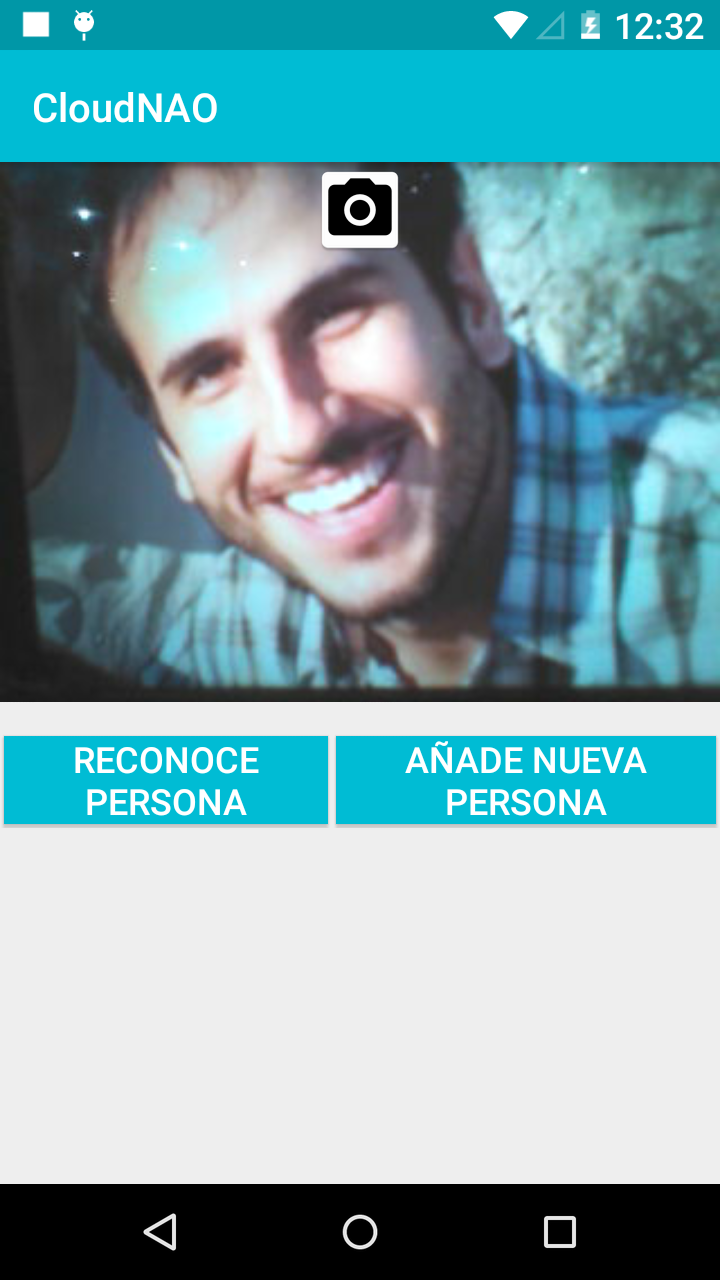
\includegraphics[scale=.1]{face_study_case1}}%
    \qquad
    \subfloat{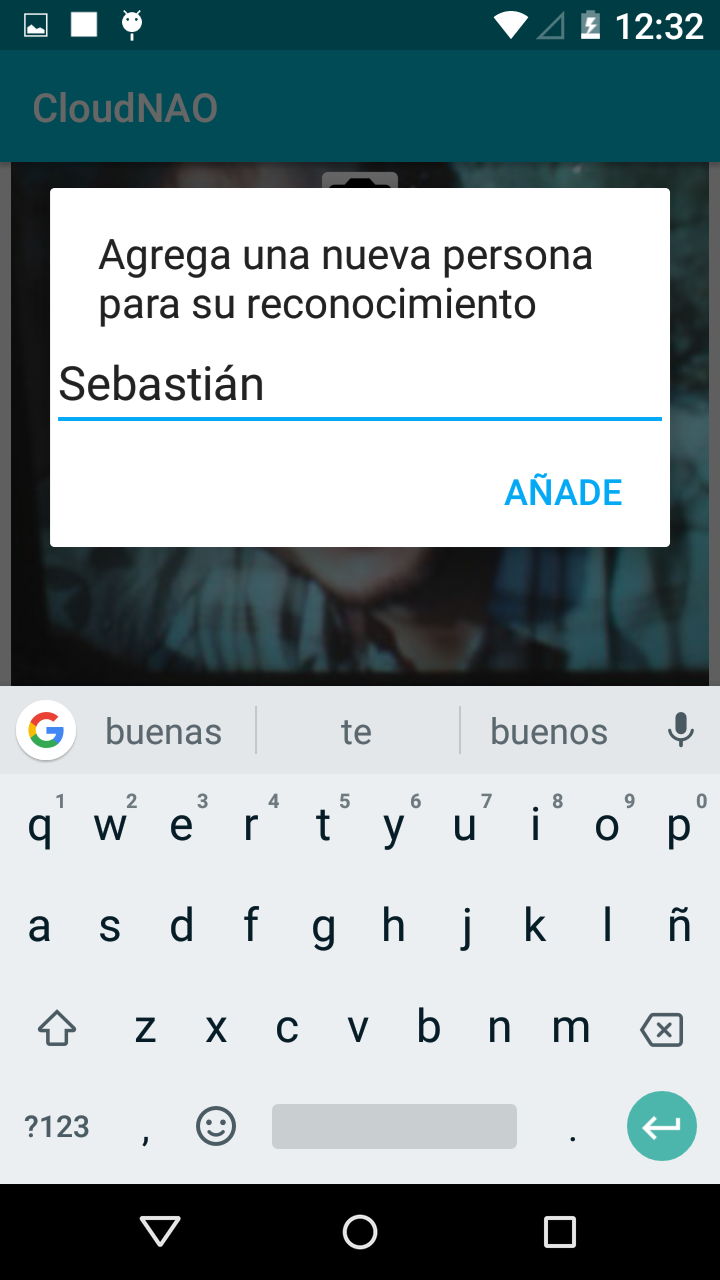
\includegraphics[scale=.1]{face_study_case2}}%
    \qquad
    \subfloat{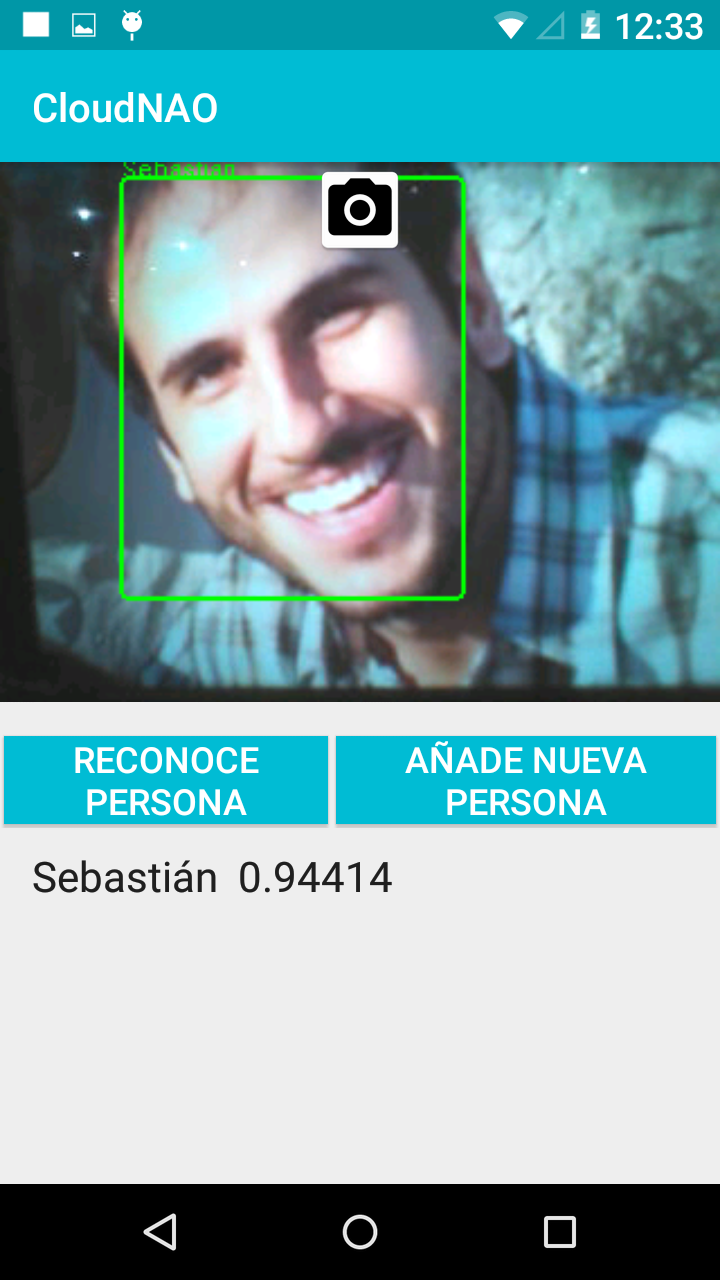
\includegraphics[scale=.1]{face_study_case3}}%
    \caption{Ejemplo de cómo se registrar un nuevo sujeto para su posterior reconocimiento.}
\end{figure}
Cuando el usuario selecciona en el menú de navegación de la aplicación
la tarea de \textbf{Reconocimiento de personas} se muestra una pantalla 
con tres botones, uno para obtener una fotografía del robot, otro para
detectar rostros de nuevas personas, y el tercero para reconocer sujetos
ya almacenados. Si el usuario desea añadir a una nueva persona, se abre un
formulario emergente con un campo para agregar el nombre de la persona y
si no hay errores y la detección se realizó correctamente,
la cara de la persona queda almacenada y se pueden realizar futuros reconocimientos.
Si se desea realizar el reconocimiento de personas cuyo rostro
fue previamente guardado, se presiona el botón con la etiqueta
\textit{Reconoce personas} y si todo sale bien,
se muestra una lista de las personas en la fotografía.
Al dar clic sobre el nombre de la persona en la lista, el robot ejecuta
un movimiento de saludo diciendo una frase simple con el nombre de la persona.



\subsubsection{Resultados}

La velocidad de la ejecución de la tarea
depende mucho de la conexión a internet.
El ejemplo en el que se ocupa el reconocimiento
de rostros es bastante sencillo, el robot
sólo hace un gesto de saludo. No obstante 
podemos añadir más funcionalidades donde
aprovechemos el análisis completo que ofrece
Kairos, la detección del género, la edad y la raza.



\begin{figure}[htbp]
\centering
\caption{El flujo de el reconocimiento de personas. 1) El usuario presiona el botón para capturar una imagen desde el robot. 2) El robot envía la imagen a la 
aplicación. 3) El usuario presiona el botón Reconoce personas y envía la imagen a la API REST. 4) La API solicita el recurso \texttt{recognize} de Kairos. 5) Kairos envía un JSON como respuesta. 6) La API 
envía un JSON a la aplicación móvil. 7) La aplicación ejecuta remotamente el módulo de NAOqi para realizar el discurso animado.}
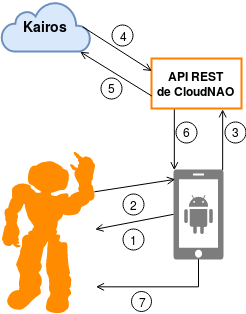
\includegraphics[scale=0.6]{study_case_kairos}
\end{figure}



\subsection{Reconocimiento óptico de caracteres y traducción de texto}

Una aplicación interesante es la
detección de texto en una imagen y su
traducción.
En la API REST se combinan dos servicios
para añadir al robot NAO la funcionalidad de extracción y traducción de texto en imágenes. 


\subsubsection{Objetivos}

\begin{itemize}
    \item Implementar el reconocimiento óptico
    de caracteres sobre el robot NAO.
    \item Utilizar servicios en la nube para traducción
    automática neuronal y reconocimiento óptico de caracteres.
    \item Permitir que el robot asista a los usuarios
    en la traducción de texto encontrado en una imagen.
\end{itemize}

\subsubsection{Problema}

El reconocimiento óptico de caracteres (OCR por sus siglas en inglés) permite detectar y extraer texto de imágenes para luego
almacenarlo en un formato que una máquina pueda entender.

A diferencia del caso de estudio anterior, el robot NAO
no cuenta con una API para detección de
texto en imágenes, ni con una herramienta
para traducir sentencias. Por las características
del robot, la interacción con humanos es 
amigable, por lo que una funcionalidad como la de asistir
a los usuarios en la traducción de texto a través
de imágenes tiene una amplia aplicación.

\subsubsection{Solución}


La API de Vision de Google Cloud ofrece el servicio de OCR
que además incluye la detección del idioma en que se encuentra escrito.
Google Cloud cuenta también con una API para traducción de 
texto.
En la API REST combinan estos dos servicios
para añadir al robot NAO la funcionalidad de extracción y traducción de texto en imágenes. 

El usuario simplemente adquiere una fotografía
capturada por la cámara del robot y se hace la petición
a la API REST que utiliza los servicios
de Google Cloud Vision y Translation para obtener el texto
y hacer la traducción, respectivamente.
Si existe texto en la imagen y fue correctamente procesado por
la API de Vision, éste se traduce, el resultado se muestra
en la aplicación y el robot repite oralmente
el texto traducido.

\subsubsection{Resultados}

Gracias a los servicios utilizados, la traducción 
del texto en una imagen se resuelve fácilmente.
La aplicación ofrece una interfaz fácil para cualquier
usuario. El tiempo de ejecución de la tarea
es de unos cuantos segundos (entre 5 aproximadamente), aunque es
una variable dependiente de la velocidad de la conexión 
a internet.


\begin{figure}[htbp]
    \centering
    \subfloat{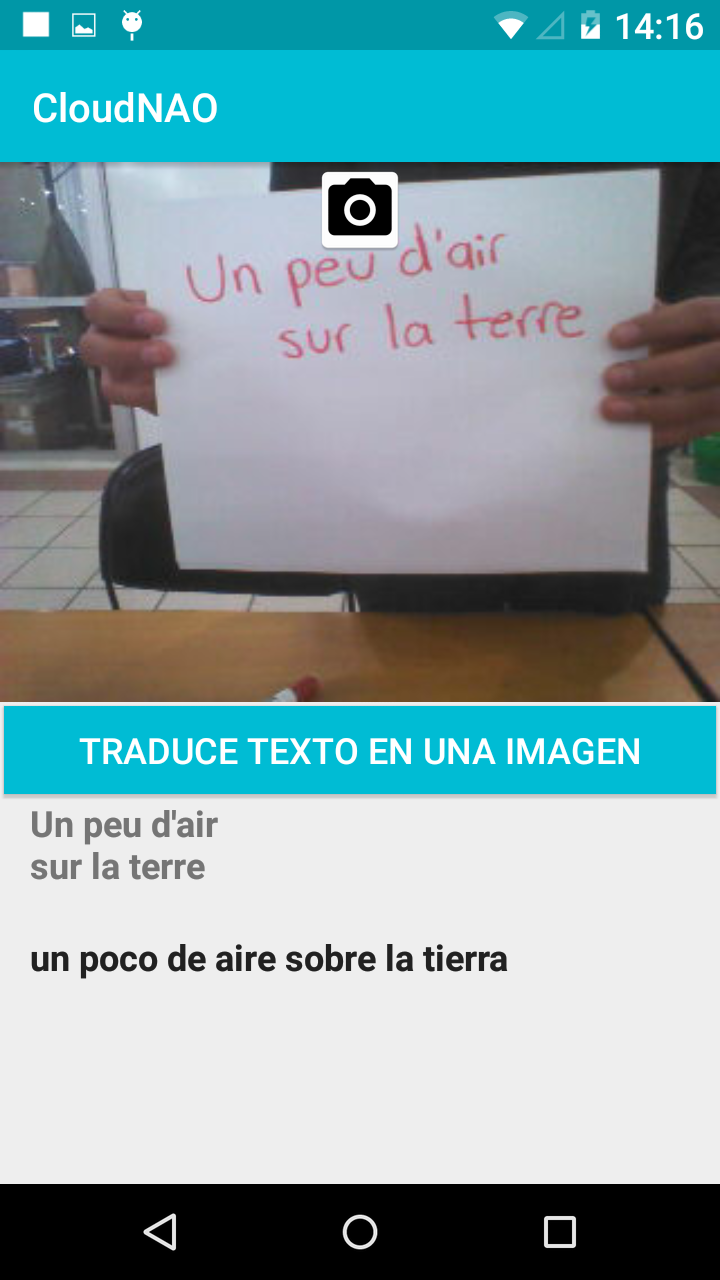
\includegraphics[scale=.1]{ocr_study_case1}}%
    \qquad
    \subfloat{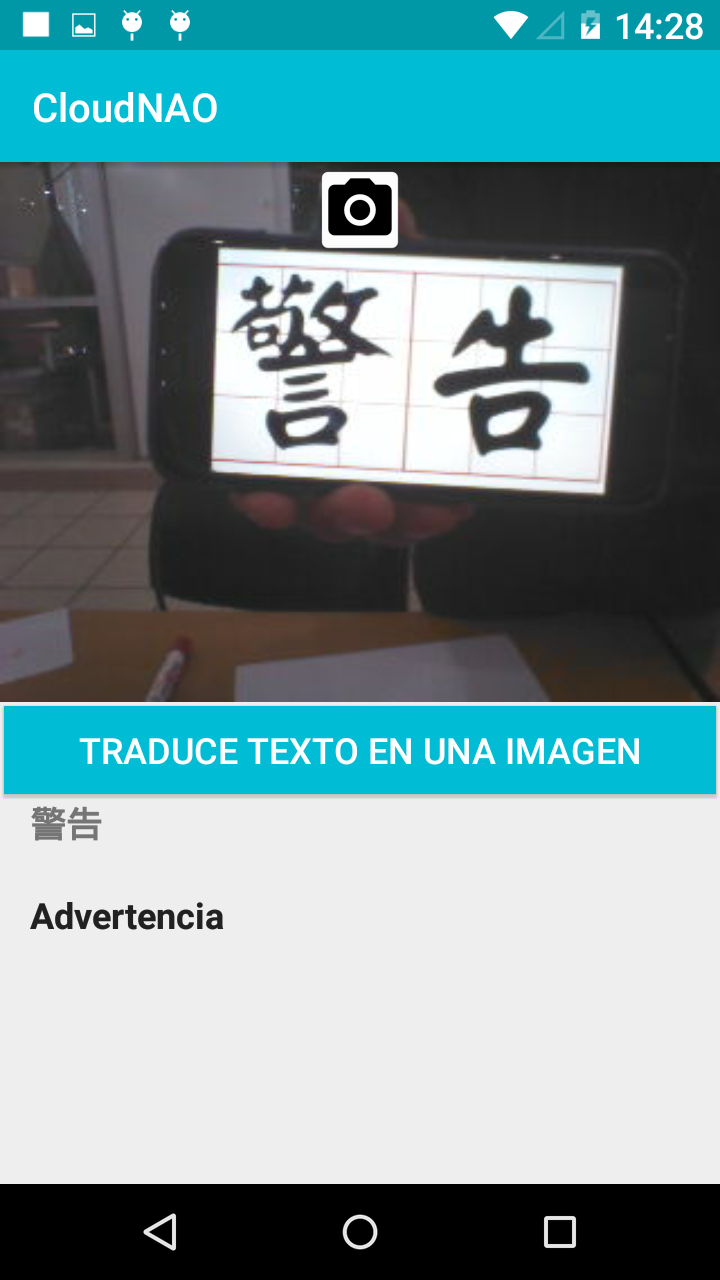
\includegraphics[scale=.1]{ocr_study_case2}}
    \caption{Ejemplo de la traducción
    de dos sentencias, la primera en francés y la segunda
    en chino.}
\end{figure}

\subsection{Reconocimiento de voz}

Este caso de estudio se aplica
directamente sobre el robot NAO, conectándolo
a la API de Wit.ai para procesamiento de
un discurso oral y poder interactuar con él a través de comandos de voz.


\subsubsection{Objetivos}

\begin{itemize}

    \item Utilizar un servicio de procesamiento
    de lenguaje natural en la nube.
    \item Desarrollar un asistente sencillo con una interacción por voz sobre el robot NAO.
    \item Implementar en el robot, un programa local
    que se conecte con servicios en la nube.
    
\end{itemize}

\subsubsection{Problema}


Una aplicación interesante de tecnologías que realizan el
procesamiento de lenguaje natural es la creación de bots conversacionales
o asistentes por voz.
El robot NAO es una plataforma con las características
para servir como asistente por voz, que a pesar de contar con un
módulo de reconocimiento de voz (\texttt{ALSpeechRecognition}), éste es muy 
básico y limitado.

Una aplicación de reconocimiento de voz
utilizando únicamente la API de NAOqi es estática.
El módulo \texttt{ALSpeechRecognition} sólo reconoce
palabras predefinidas no la intención
del discurso del usuario.f
Por ejemplo, si deseamos que el robot salude
cuando un usuario lo hace, se deben 
definir todas las formas posibles en las que
la persona puede decir "Hola".

\subsubsection{Solución}

Wit.ai provee una API para construir aplicaciones
con las que los usuarios se puedan comunicar a través de voz o texto.
Las aplicaciones desarrollados con Wit.ai aprenden conforme reciban más 
información, se vuelven más inteligentes con cada interacción de los usuarios.

Se creó una aplicación sencilla
para interactuar con el robot usando el servicio \texttt{speech} de
Wit.ai.
Dentro de la API REST existe un módulo para hacer las peticiones
a la API de Wit.ai. Éste también puede usarse directamente sobre
el robot, evitando un intermediario.
Se solicita el recurso \texttt{speech} de la API de Wit.ai 
enviando
un archivo de audio generado por el robot. La API
envía como respuesta un JSON con la transcripción del audio 
en texto, las entidades e intenciones encontradas.
El robot es quien se encarga de manejar el flujo de
acciones dependiendo de las intenciones.

Las intenciones y entidades de una aplicación se definen en la plataforma
web de Wit.ai. Ésta cuenta con una herramienta para
crear estos dos elementos a partir de oraciones que el usuario
posiblemente enviará en un mensaje. Por ejemplo,
cuando el usuario inicie una conversación posiblemente
sea con un "Hola robot", por lo que podemos definir una
intención con valor \texttt{saludo}.
Se pueden añadir más sentencias
que correspondan a la intención \texttt{saludo}
como "Buenas tardes" o
"Buena día NAO".
La entidades permite realizar específicamente cierta acción.
Por ejemplo, si le decimos "Cambia a la posición de descanso", la intención es \texttt{cambiar posición} y la
entidad es a qué posición debe cambiar, a la de descanso
en nuestro ejemplo.
A partir de esto podemos definir acciones muy simples
para el robot guiadas por las intenciones y entidades. En la tabla \ref{table:intents-study-case} se describen las intenciones y entidades que se
definieron para esta aplicación
y un ejemplo de lo que puede decir el usuario para ejecutar la acción asociada con la intención.

\begin{table}[ht]
\centering
\caption{El valor de la entidad en la sentencia
del usuario se encuentra subrayado.
\label{table:intents-study-case}}
\begin{tabular}{|l|l|l|}
\hline
Intención                                                           & Entidades                                                        & \begin{tabular}[c]{@{}l@{}}El usuario\\ puede decir ...\end{tabular}    \\ \hline
\begin{tabular}[c]{@{}l@{}}CAMBIAR\\ POSTURA\end{tabular}           & postura                                                          & \begin{tabular}[c]{@{}l@{}}Ve a la posición\\ de \underline{descanso}\end{tabular} \\ \hline
CAMINAR                                                             & dirección                                                        & \begin{tabular}[c]{@{}l@{}}Camina hacia\\ la \underline{derecha}\end{tabular}      \\ \hline
INICIO                                                              & nombre del usuario                                               & \begin{tabular}[c]{@{}l@{}}Hola NAO, me llamo\\ \underline{Ivan}\end{tabular}      \\ \hline
FIN                                                                 &                                                                  & Adiós robot                                                            \\ \hline
\begin{tabular}[c]{@{}l@{}}PROCESAMIENTO\\ DE IMÁGENES\end{tabular} & \begin{tabular}[c]{@{}l@{}}tipo de \\ procesamiento\end{tabular} & Lee el \underline{texto}                                                           \\ \hline
\begin{tabular}[c]{@{}l@{}}GUARDA\\ IMÁGENES\end{tabular}           & \begin{tabular}[c]{@{}l@{}}número de\\ fotografías\end{tabular}  & Toma \underline{diez} fotos                                                        \\ \hline
\end{tabular}
\end{table}



% \begin{itemize}
% \item  \texttt{walk}: El robot camina una pequeña distancia. "Vamos, camina."
% \item \texttt{restPosition}: El robot cambia a una posición de descanso (crouch). "Descansa robot".
% \item \texttt{greeting}: El robot realiza un gesto y saluda al usuario."Hola robot".
% \item \texttt{photography}: El robot toma una fotografía y la almacena en su disco. "Toma una foto de lo que ves".
% \item \texttt{stop}: El robot se despide del usuario va a una posición de
% descanso y termina la aplicación. "Adiós robot".
% \item \texttt{animation}: El robot ejecuta una animación aleatoria.
% "Robot, dame un movimiento sorpresa".
% \item \texttt{textDetection}: Utilizando la API de Vision de Google Cloud
% el robot extrae texto de una imagen y lo expresa oralmente. "Lee que dice
% aquí".
% \end{itemize}

\subsubsection{Resultados}

Pese a ser una aplicación muy simple
se puede volver tan compleja como se desee,
el añadir más entidades hace más interesante interactuar con el
robot. Podemos agregar otros servicios para
que cada vez se parezca más a un asistente por voz,
como los calendarios y contactos de Google, la búsqueda de lugares y
zonas de interés con servicios como Foursquare o los Mapas de Google,
uso de la la gráfica de conocimiento de Google o de Wolfram Alpha, 
servicios de noticias, etc. El robot no pone las limitaciones 
de la aplicación, ya que éste solamente es una interfaz
entre los servicios en la nube y los usuarios.

\begin{figure}[htbp]
\centering
\caption{El funcionamiento de la interacción con el robot a través de un discurso
oral. 1) El usuario envía un mensaje que el robot graba en un archivo de audio de 3 segundos de duración. 2) El robot envía el archivo binario de audio
a la API de Wit.ai. 3) Wit.ai envía un JSON con las entidades encontradas. El robot realiza una acción dependiendo de las entidades.}
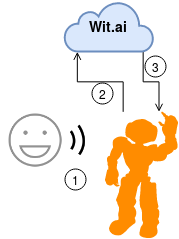
\includegraphics{study_case_wit}
\end{figure}

% \subsubsection{Clasificación de imágenes en escenarios}


% Para completar la arquitectura CloudNAO falta implementar un modelo de aprendizaje 
% profundo que se brinde como un servicio web para ser consumido por robots NAO.
% A pesar de que el servicio de detección de objetos es mantenido por el LAR, y 
% se adaptó para ser consumido a través de la API REST, no fue construido
% desde cero ya que es parte de la API de detección de objetos de TensorFlow.
% Es por eso que como parte final del proyecto se desarrolló un modelo para que 
% resuelva la tarea de clasificar imágenes.

% El problema de clasificación de imágenes es la tarea de asignarle a una imagen de
% entrada una etiqueta a partir de un conjunto de categorías. Este es uno de los principales
% problemas dentro del campo de la visión computacional, que a pesar de su simplicidad
% tiene bastantes aplicaciones prácticas. Entre esas aplicaciones, muchas interesan al
% campo de la robótica móvil, por ejemplo, para la navegación de un robot de manera
% autónoma, nos gustaría que supiera en que lugar está simplemente con una fotografía
% que obtenga en ese momento desde sus cámaras, así podría saber si ha llegado al 
% lugar de su objetivo, o a partir de la zona donde se ubica planear una trayectoria.

% Lo anterior nos inspiró en la creación de un modelo que clasificara imágenes
% de algunos lugares sobre los que podría navegar el robot NAO. 
% Como solución a este problema de clasificación se propuso usar 
% una red neuronal convolucional, que recibiera como entrada un arreglo con los
% pixeles de una imagen tomada por el robot, y la salida fuera la categoría
% a la que pertenece esa imagen. 
% Las clases en las que se desea clasificar las imágenes son lugares alrededor
% del Laboratorio de Algoritmos para la Robótica, que se ubica en el cubículo $15$ del
% Centro de Desarrollo Tecnológico de la FES Acatlán. Se eligieron las siguientes cuatro zonas:

% \begin{itemize}
%     \item El cubículo.
%     \item La salida de emergencia.
%     \item La cancha de entrenamiento de fútbol para el robot NAO.
%     \item Zona de trabajo del Laboratorio.
% \end{itemize}

\subsection{Clasificación de imágenes para localización}

Para completar la arquitectura CloudNAO falta implementar un modelo de aprendizaje 
profundo que se brinde como un servicio web para ser consumido por robots NAO.
A pesar de que el servicio de detección de objetos es mantenido por el LAR, y 
se adaptó para ser consumido a través de la API REST, no fue construido
desde cero ya que es parte de la API de detección de objetos de TensorFlow.
Es por eso que como parte final del proyecto se desarrolló un modelo para que 
resuelva la tarea de clasificar imágenes.

El problema de clasificación de imágenes es la tarea de asignarle a una imagen de
entrada una etiqueta a partir de un conjunto de categorías. Este es uno de los principales
problemas dentro del campo de la visión computacional, que a pesar de su simplicidad
tiene bastantes aplicaciones prácticas. Entre esas aplicaciones, muchas interesan al
campo de la robótica móvil, por ejemplo, para la navegación de un robot de manera
autónoma, nos gustaría que supiera en que lugar está simplemente con una fotografía
que obtenga en ese momento desde sus cámaras, así podría saber si ha llegado al 
lugar de su objetivo, o a partir de la zona donde se ubica planear una trayectoria.

Lo anterior nos inspiró en la creación de un modelo que clasificara imágenes
de algunos lugares sobre los que podría navegar el robot NAO. 
Como solución a este problema de clasificación se propuso usar 
una red neuronal convolucional, que recibiera como entrada un arreglo con los
pixeles de una imagen tomada por el robot, y la salida fuera la categoría
a la que pertenece esa imagen. 
Las clases en las que se desea clasificar las imágenes son lugares alrededor
del Laboratorio de Algoritmos para la Robótica, que se ubica en el cubículo $15$ del
Centro de Desarrollo Tecnológico de la FES Acatlán. Se eligieron las siguientes cuatro zonas:

\begin{itemize}
    \item El cubículo.
    \item La salida de emergencia.
    \item La cancha de entrenamiento de fútbol para el robot NAO.
    \item Zona de trabajo del Laboratorio.
\end{itemize}

Para finalizar,
se debe integrar uno de los cinco modelos descritos en la tabla \ref{table:models_results} sobre la API REST de CloudNAO y luego hacer peticiones con el robot a ésta.
Los modelos elaborados en TensorFlow contienen la gráfica de cómputo
y los valores de los parámetros que se han entrenado. Estos datos
están contenidos en varios archivos que se pueden guardar para
entrenamientos posteriores o para realizar inferencias sobre 
un modelo cuyas variables han sido aprendidas.

Se eligió el modelo con la precisión más alta y con el menor
tiempo de entrenamiento que es el modelo (1). 
%Durante la ejecución
%de la gráfica del modelo se crea una instancia de la clase \texttt{tf.train.Saver()}. Esto crea cuatro archivos
%uno con extensión \texttt{.meta}, uno con extensión \texttt{.index},
%otro con extensión \texttt{.data} y otro sin extensión llamado
%\texttt{checkpoint}. El primero guarda toda la gráfica de
%TensorFlow, los otros tres almacenan los valores de las variables.
%Después de guardar, simplemente se restaura el modelo
%y se puedan hacer inferencias al alimentarlo con una imagen.
Dentro de la API REST, la clase que se encarga de restaurar la gráfica y valores del modelo
es \texttt{ImageClasssfier} dentro del módulo \texttt{indoor\_scenes\_classsifier} del paquete \texttt{tf\_models}.
En el apartado \textit{Modelos de TensorFlow (tf\_models)}
de la sección \ref{chapter_two/desc_cloudnao:api-rest-de-cloudnao}
se describe cómo utilizar esta clase.

Por otra parte el robot NAO o cualquier otro
dispositivo cliente se comunica con la API a través
de una biblioteca que permita hacer peticiones 
HTTP. En el caso del robot ocupamos la biblioteca
\texttt{requests} de Python. Para obtener una imagen 
del robot codificada en base 64 se utilizó la clase \texttt{Robot}
del módulo \texttt{nao\_robot} descrito en la sección
\ref{\detokenize{firebase-nao-robot}}. Es la cadena
que representa la imagen la que se envía a la API REST usando
\texttt{requests}.

Se hicieron $40$ solicitudes a la API REST desde el robot,
$10$ por cada categoría. Esto es, se enviaron
$10$ imágenes de la cancha, $10$ de la salida,
$10$ del cubículo y $10$ del área de trabajo.
En las tablas \ref{table:soccer_nao_results},
\ref{table:exit}, \ref{table:desks} y
\ref{table:office}, se resumen los resultados obtenidos.
En la figura \ref{nao_api_images} se muestran algunas imágenes capturadas en las pruebas.



Se puede ver que existen más aciertos
con imágenes de la cancha de fútbol, 8 de 10 inferencias correctas.
Clasificando imágenes de la salida de emergencia
y del cubículo se tienen 7 de 10 predicciones correctas.
Para el área de trabajo tuvo su peor desempeño con 6 de
10 aciertos. Si bien no se obtiene
la precisión reportada durante el
entrenamiento del modelo, el tiempo
de ejecución y los
resultados son buenos
para la funcionalidad de
auxiliar a la navegación del robot.
El tiempo de solicitud y repuesta varía entre peticiones.
Factores que influyen al tiempo son el tamaño de la 
imagen enviada y la velocidad de la conexión del cliente
y del servidor. Convendría probar el modelo sobre PaaS
como Google Cloud o Heroku para ver si hay una mejora
en el tiempo.



\begin{table}[!h]
\centering
\begin{tabular}{|l|l|l|l|}
\hline
Clase        & Predicción   & Tiempo        & Correcta \\ \hline
cancha & z. trabajo        & 3.0337650776 & F        \\ \hline
cancha & cancha & 3.0559039116 & T        \\ \hline
cancha & z. trabajo        & 2.09687018394 & F        \\ \hline
cancha & cancha & 3.0169699192 & T        \\ \hline
cancha & z. trabajo        & 2.32713413239 & F        \\ \hline
cancha & cancha & 3.0284428596 & T        \\ \hline
cancha & cancha & 3.0252449512 & T        \\ \hline
cancha & cancha & 3.1204240322 & T        \\ \hline
cancha & cancha & 3.013076067  & T        \\ \hline
cancha & cancha & 3.2163701057 & T        \\ \hline
\end{tabular}
\caption{Resultados de las imágenes de la cancha de fútbol.}
\label{table:soccer_nao_results}
\end{table}

\begin{table}[!h]
\centering
\begin{tabular}{|l|l|l|l|}
\hline
Clase & Predicción & Tiempo        & Correcta \\ \hline
salida  & salida       & 3.2262349129 & T     \\ \hline
salida  & salida       & 3.0402858257 & T     \\ \hline
salida  & salida     & 3.298979044  & T    \\ \hline
salida  & cubículo     & 3.6488580704 & F    \\ \hline
salida  & salida       & 3.4767799377 & T     \\ \hline
salida  & salida       & 3.6147930622 & T     \\ \hline
salida  & salida       & 3.7430388927 & T     \\ \hline
salida  & cubículo     & 3.7496609688 & F    \\ \hline
salida  & salida       & 3.8713350296 & T     \\ \hline
salida  & cubículo     & 4.0420210361 & F    \\ \hline
\end{tabular}
\caption{Resultados para fotografías de la salida de emergencia.}
\label{table:exit}
\end{table}

\begin{table}[!h]
\centering
\begin{tabular}{|l|l|l|l|}
\hline
Clase      & Predicción & Tiempo        & Correcta \\ \hline
z. trabajo & z. trabajo & 5.3504459858 & T        \\ \hline
z. trabajo & cubículo    & 5.2893049717 & F        \\ \hline
z. trabajo & cubículo    & 5.2149860859 & F        \\ \hline
z. trabajo & z. trabajo & 5.2179970741 & T        \\ \hline
z. trabajo & cubículo    & 5.6882929802 & F        \\ \hline
z. trabajo & cubículo    & 5.6848390102 & F        \\ \hline
z. trabajo & z. trabajo & 5.9792921543 & T        \\ \hline
z. trabajo & z. trabajo & 5.8859920502 & T        \\ \hline
z. trabajo & z. trabajo & 5.722206831  & T        \\ \hline
z. trabajo & z. trabajo & 6.7581658363 & T        \\ \hline
\end{tabular}
\caption{Resultados para la fotografías del área
de trabajo.}
\label{table:desks}
\end{table}

\begin{table}[!h]
\centering
\begin{tabular}{|l|l|l|l|}
\hline
Clase   & Predicción & Tiempo        & Correcta \\ \hline
cubículo & cubículo    & 3.5342819691 & T        \\ \hline
cubículo & cubículo    & 3.9999611378 & T        \\ \hline
cubículo & z. trabajo & 4.6536300182 & F        \\ \hline
cubículo & z. trabajo & 3.8637499809 & F        \\ \hline
cubículo & z. trabajo & 4.887745142  & F        \\ \hline
cubículo & cubículo    & 4.4888358116 & T        \\ \hline
cubículo & cubículo    & 4.6198430061 & T        \\ \hline
cubículo & cubículo    & 4.4448840618 & T        \\ \hline
cubículo & cubículo    & 4.5735599995 & T        \\ \hline
cubículo & cubículo    & 5.2998209    & T        \\ \hline
\end{tabular}
\caption{Resultados de obtenidos con imágenes del cubículo.}
\label{table:office}
\end{table}

\begin{figure}[!ht] 
  \centering
\subfloat[Clase = cancha, predicción = cancha. Tiempo = 3.05]{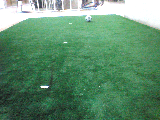
\includegraphics[scale=1]{nao_api_soccer}}
\qquad
\subfloat[Clase = salida, predicción = salida. Tiempo = 3.29]{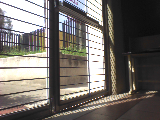
\includegraphics[scale=1]{exit_incorrect}}
\qquad
\subfloat[Clase = zona de trabajo, predicción = cubículo. Tiempo = 5.21]{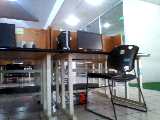
\includegraphics[scale=1]{deks_incorrect}}
\qquad
\subfloat[Clase = cubículo, predicción = cubículo. Tiempo = 3.53]{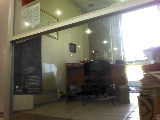
\includegraphics[scale=1]{nao_api_office}}
\caption{Predicciones hechas enviando imágenes del robot a la API REST. El tiempo son los
segundos que se tardó en enviar la solicitud y en recibir la respuesa. \label{nao_api_images}}
\end{figure}

%\section{Resultados}
\section{Conclusiones}


El objetivo principal de esta tesis fue 
que el robot Fibonacho
utilizará tecnologías emergentes como son el cómputo en la nube
y el aprendizaje 
profundo.
Cualquier dispositivo que pueda solicitar y
manejar mensajes HTTP puede hacer uso de los servicios
de la API REST.
Como nota final puedo decir que las tecnologías empleadas
facilitan la adición
de nuevas funcionalidades sobre una plataforma con recursos
limitados, como los son los robots NAO,
permitiendo introducir al robot a otros campos de estudio.
% En la aplicación
% móvil se muestran algunos casos de uso del consumo de
% servicios para que el robot NAO pueda realizar tareas
% que por su capacidad de procesamiento no podría 
% llevar a cabo de manera autónoma.
% Con ésta, el robot puede generar datos que
% se guardan en la nube o tomar una fotografía,
% enviarla a un servicio para su procesamiento y a partir
% de la respuesta obtenida realizar una acción; todo
% esto en cuestión de segundos.
% Sin embargo, un problema pendiente de la aplicación móvil
% es la compatibilidad del SDK de NAOqi con nuevos sistemas
% Android.

% El papel de Firebase es importante porque muestra
% los principales beneficios de la nube en el desarrollo
% de aplicaciones modernas. Cuenta con una base de datos en tiempo
% real que permite mandar comandos al robot de manera
% inmediata, almacenar grandes volúmenes de datos
% producidos por los sensores de éste y sincronizarlos entre los dispositivos
% conectados.

% Otra parte fundamental del trabajo fue el desarrollo
% de una red neuronal convolucional para la clasificación
% de imágenes en diferentes escenarios dentro del laboratorio.
% De la experimentación, encontramos modelos
% cuyo tiempo de entrenamiento es relativamente bajo, sólo unos 
% cuantos pares de minutos, y cuya precisión es muy alta, que 
% aunque no significa que sean excelentes clasificadores,
% las pruebas sobre el robot funcionaron bien.
% Esto en parte se debe a que
% TensorFlow hace simples y eficientes
% la definición, el entrenamiento y la carga de modelos de 
% aprendizaje automático. 
% Un trabajo a futuro sería desarrollar un caso de estudio 
% donde el modelo sirva como auxiliar en la navegación
% del robot.


\nocite{*}
\bibliographystyle{unsrt}
\bibliography{referencias}
\end{document}
